\chapter{The Monomorphic Interpreter}
\label{chapter:implementation}
% \epigraph{Typing is no substitute for thinking.}{Dartmouth Basic manual, 1964}

This chapter will describe the methods used to transform TASTy to make it suitable for a Truffle interpreter, \textsc{TastyTruffle}, \textit{without} polymorphism.
In particular, it will cover how to translate the organization of data and code in the \scalainline{DefDef}, \scalainline{ClassDef}, and \scalainline{Term} tree nodes into a Truffle implementation, which is amenable to execution and JIT optimization.
Chapter \ref{implementation:specialization} will then discuss extensions to our implementation to support parametric polymorphism and cover the techniques we use to specialize nodes to eliminate autoboxing in the presence of polymorphism. 

Scala programs in TASTy format are unsuitable for execution in a Truffle interpreter. 
Programs in TASTy must be parsed and transformed into an executable representation in Truffle.
These transformations translate the TASTy tree structure into a more straightforward but semantically equivalent Truffle AST.
For the rest of this thesis, we refer to the Truffle AST of TASTy as \textit{TastyTruffle IR}.
As TASTy represents a Scala program close to its equivalent source representation, canonicalization compiler passes (see appendix \ref{appendix:dotty-phases}) that would otherwise normalize the IR are not present. 
Instead, we implement TastyTruffle IR to represent a canonicalized executable intermediate representation that can later be specialized on demand. 

\begin{figure}[!htb]
	\begin{minted}{scala}
	def parseTopLevel(tree: Tree): Object = tree match {
		case vdef: ValDef   => 
			lazy val obj = initializeObject(vdef)
			registerObject(vdef.symbol, obj)			
		case cdef: ClassDef => 
			registerShape(cdef.tpe, parseClassDef(cdef))	
		case _ => ()
	}
	\end{minted}
	\caption{Pseudocode to evaluate every top level tree.}
	\label{impl:top-level}
\end{figure}

Figure \ref{impl:top-level} gives an evaluation loop typical in other interpreters in the context of this one.
A top-level tree is any tree without a parent.
In our subset of TASTy, a top level tree may be a \scalainline{ValDef} (a singleton object) or a \scalainline{ClassDef}.
Here we only present the pseudocode sufficient to traverse a program in TASTy. 
Each top-level definition is parsed and saved in a global interpreter context (\scalainline{registerShape} and \scalainline{registerObject}).
Top-level objects are lazily initialized as their class definitions may not have been parsed.
Registered objects and classes are then used in subsequent executions of the program.

We omit details on \textit{how} to execute the program to be concise.
Entry points in \scalainline{TASTy} are defined by a special method \scalainline{main}.
As multiple entry points may exist in a given program, we consider the selection of entry points as an implementation-specific detail.
In the following sections, we will describe the individual types of TASTy nodes, why some are directly unsuitable for execution, and how to simplify their semantics.

\section{Converting the \texttt{DefDef} tree into a Truffle \texttt{RootNode}}
\label{impl:subsection:defdef}

In this section, we describe the conversion of \scalainline{DefDef} trees to \textit{root nodes}.
\scalainline{DefDef} trees are the primary structure that organizes code (terms) in TASTY.
Root nodes represent the root of an executable Truffle AST, the primary abstraction that organizes code in Truffle.
In our case, root nodes are the Truffle analog of a \scalainline{DefDef}.
Each root node has a corresponding \textit{call target}, which is used for the invocation of the root node.
Call targets are the primary compilation unit for Graal.
A compilation unit is an organization of code that can be independently compiled.
A root node is automatically instrumented\cite{profiling:atom} to profile its number of invocations. 
When a root node has been frequently invoked inside the interpreter, it is JIT compiled into machine code by Graal.
Subsequent invocations of the call target will then use the more efficient compiled root node.

\begin{figure}[!htb]
\begin{minted}{scala}
abstract class RootNode(desc: FrameDescriptor) {
	def execute(frame: VirtualFrame): Object
	def getCallTarget: CallTarget
}
\end{minted}
\caption{Pseudocode of a root node.}
\label{example:root-node}
\end{figure}

Figure \ref{example:root-node} gives a simplified implementation of a root node.
Each root node in Truffle has a \textit{frame descriptor} and execution semantics.
A guest language must subclass and implement its root node to enable function invocation semantics.

A frame descriptor describes guest language variables that are in scope during execution.
The abstract \javainline{execute} method describes the invocation behaviour of a root node.
When a root node is executed, it is always supplied with a \textit{frame}.
A frame contains the arguments supplied during invocation and storage slots for local variable definitions in the body of the method.

\begin{figure}[!htb]
\begin{minted}{scala}
class DefDef(
	_: String, 
	params: List[ParamClause], 
	_: TypeTree, 
	rhs: Option[Term]) extends Definition	
\end{minted}
\caption{Definition of a \texttt{DefDef} tree with names of less important members replaced with \texttt{\_}}
\label{recall:defdef}
\end{figure}

A further simplified definition of a \scalainline{DefDef} tree is provided in figure \ref{recall:defdef}.
This section focuses on two members of a \scalainline{DefDef} tree.
The parameters of a \scalainline{DefDef} tree are given by the \scalainline{params} field.
In practice, the type of a \scalainline{ParamClause} is an alias for the union type \scalainline{TypeParams {|} TermParams}, so we omit the \scalainline{ParamClause} definition.
A \scalainline{DefDef} tree will have a parameter section for type parameters when they are polymorphic and will always have a term parameters section.
\scalainline{DefDef} trees may optionally have a body defined in the \scalainline{rhs} field.
When trees do not have a body defined, they are abstract method definitions and do not have a corresponding root node in Truffle.
Only non-abstract method definitions with a body (a term) are executable.
The explanation f parsing of terms into nodes for execution is given in section \ref{impl:subsection:classdef}

\begin{figure}[!htb]
\begin{minted}{scala}
object FrameSlotKind extends Enumeration {
	type FrameSlotKind = Value
	val Object, Long, Int, Double, Float, Boolean, Byte = Value
}	
	
def getFrameSlotKind(tpe: Type): FrameSlotKind = 
	if (tpe.isPrimitive) 
		// Int => FrameSlotKind.Int
		// ...
		// Double => FrameSlotKind.Double
		getPrimitiveSlotKind(tpe)
	else  
		FrameSlotKind.Object
\end{minted}
\caption{Simplified implementation of \scalainline{FrameSlotKind}}
\label{impl:frameslot-kind}
\end{figure}

Each value definition in the parameters of a \scalainline{DefDef} will have a corresponding frame slot in its parent frame descriptor. 
A frame slot references a unique frame value in the context of a root node.
Truffle permits each frame slot in a frame descriptor to be described by a \textit{frame slot kind}.
In Truffle, there is a corresponding frame slot kind for reference types and each JVM primitive type. 
The pseudocode of a frame slot kind and a method to convert a type into a slot kind is given in \ref{impl:frameslot-kind}.

Truffle profiles frame accesses to minimize the amount of autoboxing that occurs when reading from a frame slot with an \javainline{Object} kind. 
To eliminate unnecessary specialization of frame accesses where types are monomorphic and statically refer to a primitive type, a parameter is assigned the matching primitive frame slot kind in the frame descriptor. 
In cases where the type is not a primitive type or a polymorphic applied type, e.g. \scalainline{List[T]} but not \scalainline{T}, The \scalainline{Object} kind is assigned to the frame slot.
Otherwise, the type is a polymorphic parameter, which \textit{could} resolve to a primitive type, and the frame slot kind cannot be resolved statically.
We will defer discussion on handling parameters of such polymorphic types that cannot be resolved statically until section \ref{implementation:specialization}.

\begin{figure}[!htb]
\begin{minted}{scala}
case class LocalFrameVal(slot: FrameSlot, kind: FrameSlotKind)
	
class DefDefNode(
	desc: FrameDescriptor, 
	params: Array[LocalFrameVal], 
	body: TermNode) extends RootNode(desc) {
	override def execute(frame: VirtualFrame): Object = {
		copyArgumentsToFrame(frame)
		try {
			body.execute()
		} catch {
			case ex: ReturnException => ex.getValue
		}
	}	
		
	def copyArgumentsToFrame(frame: VirtualFrame): Unit = 
		for ((param, arg) <- params zip frame.getArguments) 
			param.kind match {
				case FrameSlotKind.Int =>
					frame.setInt(param.slot, arg.asInstanceOf[Int])
				...
				case FrameSlotKind.Double =>
					frame.setDouble(param.slot, arg.asInstanceOf[Double])	
				case _ =>
					frame.setObject(param.slot, arg)
			}
}
\end{minted}
\caption{Pseudocode for \scalainline{DefDefNode} and \scalainline{Parameter}}
\label{impl:defdefnode}
\end{figure}

Figure \ref{impl:defdefnode} provides the implementation of the \scalainline{DefDefNode} and its parameters, the root node equivalent of a \scalainline{DefDef}.
The execution of a \scalainline{DefDefNode} is divided into two stages, argument preparation, and execution.
First, the arguments of the frame constructed during invocation (see \ref{impl:subsection:apply}) are copied into their respective parameter frame slots.
Frames contain separate regions for values of each frame slot kind.
We copy each argument into the appropriate frame slot region based on the frame slot kind prescribed to a parameter.
Storing parameters in this manner eliminates any unnecessary boxing that would otherwise occur when passing primitives as arguments.

By default, all frames start off \textit{virtual}.
Virtual frames are Truffle abstractions that provide guest languages an opportunity to exploit escape analysis.
Escape analysis\cite{escape-analysis} reasons about the dynamic scope of object allocations. 
Truffle and Graal both exploit the observations of \textit{Partial Escape Analysis}\cite{java:partial-escape-analysis}, a path-sensitive variant of escape analysis, to enable the following optimizations for guest languages:

\begin{description}
	\item[Region Allocation\cite{java:escape-analysis,tofte:region-memory}] The substitution of heap allocations with stack allocations to eliminate unnecessary garbage collection.
	\item[Scalar Replacement\cite{java:escape-analysis-optimizations}] The complete elimination of an object allocation, where the fields of the replaced object are substituted by local variables.
\end{description}

\begin{figure}[!htb]
\begin{minted}{scala}
def parseDefDef(ddef: DefDef): DefDefNode = {
	val desc = new FrameDescriptor
	val parameters = self :: ddef.params.map {
		case vdef: ValDef => generateLocal(vdef, desc)
	}
		
	val body = parse(ddef.rhs)
	new DefDefNode(desc, parameters, body)
}
	
def generateLocal(vdef: ValDef, desc: FrameDescriptor): LocalFrameVal = {
	val kind = getFrameSlotKind(vdef.tpt.tpe)
	val slot = desc.addSlot(kind)
	Parameter(slot, kind)
}
\end{minted}
\caption{Pseudocode for parsing \scalainline{DefDef} into \scalainline{DefDefNode}}
\label{impl:parse-defdef}
\end{figure}

The virtual frame abstraction allows guest languages to read and write to a frame without the requirement to optimize their object allocations.
Instead, escape analysis and scalar replacement are responsible for optimizing guest language object allocations during partial evaluation. 
After arguments are copied into the frame, their values become available for access during the execution of the body.
The body of a \scalainline{DefDefNode} is then executed, and its computed value is returned.

Figure \ref{impl:parse-defdef} provides a summary on parsing a \scalainline{DefDef} tree into its Truffle equivalent \scalainline{DefDefNode}.
Frame slot and frame slot kinds provide an abstraction for parameters and arguments to be resolved before executing the main body in a \scalainline{DefDefNode}.
In addition to the parameters explicitly present in TASTY, the root node will have an additional parameter representing the method's receiver.
The receiver is an object instance whose class definition owns the method being invoked.
In Scala, every method invocation has a receiver.
In TASTy, this translates to every \scalainline{DefDef} is owned by a \scalainline{ClassDef}.
In the next section, we detail how to organize call targets in Truffle by using \scalainline{ClassDef} trees.

\section{Deriving a \texttt{Shape} from a \texttt{ClassDef}}
\label{impl:subsection:classdef}

A \scalainline{ClassDef} tree defines the layout of an object in TASTy.
The layout of an object dictates the values that an object instance stores and the methods that can be invoked on an object instance.
The data layout of an object in a Truffle interpreter is described by a \textit{shape}\cite{self:prototypes,truffle:object-model}.
A Shape is a language-agnostic model for defining the properties of an object instance in Truffle.
A property in a shape describes one member of an object instance; it has an identifier and a value.
A Truffle object instance consists of \textit{object storage}, which contains instance-specific data and its shape.
Shapes map property identifiers to object storage locations; guest languages interface with object storage indirectly through properties.
In this thesis, we use a \textit{static shape}, an immutable variant of a shape.
Normally, shapes are mutable, and their list of properties may change throughout the lifetime of a program\cite{truffleruby:object-model}.
However, programs that dynamically change the layout of their objects\cite{java:reflection} are beyond the scope of this thesis.

\begin{figure}[!htb]
\begin{minted}{scala}
class ClassDef(
	name:        String,
	constructor: DefDef, 
	parents:     List[Tree], 
	_:           Option[ValDef], 
	body:        List[Statement]
) extends Definition

class ClassShape(
	symbol:  Symbol,
	parents: Array[Symbol],
	fields:  Array[Field]
	methods: Map[MethodSignature, CallTarget]
	vtable:  Map[MethodSignature, Symbol]
) extends Shape
\end{minted}
\caption{Pseudocode of \scalainline{ClassDef} and a shape for a \scalainline{ClassDef}.}
\label{impl:class_shape}
\end{figure}

Recall the definition of a \scalainline{ClassDef} in figure \ref{impl:class_shape}.
Each \scalainline{ClassDef} tree can be transformed into a corresponding \scalainline{ClassShape}, given in figure \ref{impl:class_shape}.
Figure \ref{impl:parse-classdef} provides a very simplified implementation of the steps to transform a \scalainline{ClassDef} into a \scalainline{ClassShape}.
The \scalainline{name} parameter of \scalainline{ClassDef} alone is insufficient to be used as an identifier for a \scalainline{ClassShape}.
Names do not disambiguate between classes of the same name declared in different packages.
Instead, we used the symbol of the \scalainline{ClassDef} tree as the identifier for the \scalainline{ClassShape}.
For the remainder of this thesis, we will use a \scalainline{ClassInstance} to refer to an object instance with properties described by a \scalainline{ClassShape}.

\begin{figure}[!htb]
\begin{minted}{scala}
def parseClassDef(cdef: ClassDef): ClassShape = {
	val parents = cdef.parents.map(_.symbol)
	
	val fields = cdef.body map {
		case vdef: ValDef => generateField(vdef)	
	}
	
	val methods = (cdef.constructor :: cdef.body) map {
		case ddef: DefDef => ddef.symbol.signature -> parseDefDef(ddef)
	}
	
	val vtable = cdef.symbol.methodMembers map {
		symbol => symbol.signature -> symbol
	}

	new ClassShape(cdef.symbol, parents, fields, init ++ methods, vtable)
}

def generateField(vdef: ValDef): Field = vdef match {
	case ValDef(_: String, tpt: TypeTree, rhs: Option[Term]) => 
		new Field(vdef.symbol, vdef.tpt.tpe)
}
\end{minted}
\caption{Pseudocode to convert a \scalainline{ClassDef} into a \scalainline{ClassShape}.}
\label{impl:parse-classdef}
\end{figure}

A \scalainline{ValDef} tree in the \scalainline{ClassDef} body translates to a field definition in the \scalainline{ClassShape}.
A \scalainline{ClassShape} has a collection of fields that implement the static shape property.
Figure \ref{impl:field} gives our implementation of a field.
Fields define operations to read and write from the object storage on a \scalainline{ClassInstance}.
Like frames with frame slot kinds, object instances in Truffle have separate regions for storing values of each primitive type and one for reference types.
Following the same rules with types and frame slot kinds described in section \ref{impl:subsection:defdef}, the data access of a field depends on the type of the \scalainline{ValDef} tree from which the field originates.
The remaining members of a \scalainline{ClassShape} do not describe data that has to be stored in the object storage of a \scalainline{ClassInstance}.

\begin{figure}[!htb]
\begin{minted}{scala}
class Field(symbol: Symbol, tpe: Type) extends StaticProperty {
	override def getId: String = symbol.name
	
	def get(instance: Object): Any = 
		if (tpe == Int) getInt(instance)
		else if ...
		else if (tpe == Double) getDouble(instance)
		else getObject(instance)
	
	def set(instance: Object, value: Any): Unit = 
		if (tpe == Int) setInt(instance, value.asInstanceOf[Int])
		else if ...
		else if (tpe == Double) setDouble(instance, value.asInstanceOf[Double])
		else setObject(instance, value)	
} 
\end{minted}
\caption{Pseudocode of the field property.}
\label{impl:field}
\end{figure}

After the constructor and the \scalainline{DefDef} statements of a \scalainline{ClassDef} are converted into root nodes, they are stored in the \scalainline{ClassShape} mapped by a method signature.
The pseudocode for a method signature is given in figure \ref{impl:method-signature}.
Method signatures disambiguate method invocations in the presence of \textit{overloading}\cite{strachey:fundamental-concepts}, where methods share the same name but have different arguments.
When combined with parametric polymorphism, method signatures must also be able to disambiguate between methods sharing the same name but having different type parameters.
However, method signatures do not have to disambiguate between different type parameters by name, only the number of type parameters a method has.
Because type erasure erases polymorphic type parameters from methods, generic methods that share the same number of type parameters, as well as the same parameter types, will conflict and therefore are invalid.
As previously mentioned, methods are shared among all \scalainline{ClassInstance} objects with the same shape; call targets are stored on their owning shape.

\begin{figure}[!htb]
\begin{minted}{scala}
case class MethodSignature(symbol: Symbol, params: Int, types: Array[Type])
\end{minted}
\caption{Pseudocode of a method signature.}
\label{impl:method-signature}
\end{figure}

Often a shape will not contain the call target referenced by a signature because the dispatch is dynamic, and the original type inherits the method.
A \scalainline{ClassShape} contains a \textit{virtual method table}, which maps a method signature to the symbol of a shape that contains the call target matching the signature.
If a method signature does not have a call target in the current shape, the shape which holds the target is indirectly resolved using the virtual method table during execution.
While this resolution carries significant performance overhead in Truffle and other programming language implementations, we will describe a technique that partially mitigates this overhead further in chapter \ref{implementation:specialization}.

\section{Transforming \texttt{Terms} into \texttt{Nodes}}

\begin{figure}[!htb]
\begin{minted}{scala}
abstract class TermNode extends Node with InstrumentableNode {

	def execute(frame: VirtualFrame): Object 
	def executeInt(frame: VirtualFrame): Int = execute(frame).asInstanceOf[Int]
	...
	def executeDouble(frame: VirtualFrame): Double = execute(frame).asInstanceOf[Double]

}
\end{minted}
\caption{Pseudocode of a TermNode.}
\label{impl:term-node}
\end{figure}

In this section, the conversion of \scalainline{Term} trees into Truffle nodes is given.
The Truffle \scalainline{Node} abstraction allows guest languages to implement executable fragments of an AST.
Figure \ref{impl:term-node} is our subclass of a Truffle \scalainline{Node}.
Subclasses of the \scalainline{TermNode} will define node-specific semantics encapsulating a particular functionality of the interpreter.
The \scalainline{TermNode} takes advantage of Truffle's autoboxing elimination by defining companion \scalainline{execute[TYPE]} methods to allow subclasses to declare when an expected result from a child node must conform to a specific primitive type.
In the following sections, we give the subclasses that individually implement the monomorphic interpreter's functionality.

\subsection{Creating Instances}

\begin{figure}[!htb]
\begin{minted}{scala}
def parseNew(new: New): NewNode = new NewNode(new.tpe.symbol)	

class NewNode(symbol: Symbol) extends TermNode {
	override def execute(frame: VirtualFrame): Object =  shapeOf(symbol.tpe).newInstance
}
\end{minted}
\caption{Pseudocode of a \scalainline{NewNode} and how it is parsed.}
\label{impl:new-node}
\end{figure}

The \scalainline{New} tree represents the allocation of an instance of a \scalainline{ClassDef}.
The Truffle equivalent allocate node given in figure \ref{impl:new-node} is not so different, but it allocates an instance with properties described by the \scalainline{ClassShape} instead of a \scalainline{ClassDef}.
Note that a \scalainline{NewNode} only \textit{creates} an object; the parameters and fields of an object remain uninitialized.
An object is \textit{initialized} when the type constructor, \scalainline{<init>}, is invoked on a newly created object.
TASTy is emitted with this sequence of events in mind; object creation is always followed by object construction.
Structurally, this means that a \scalainline{New} tree is always the child of an initializer \scalainline{Apply} tree.

\subsection{Function Application}
\label{impl:subsection:apply}

\begin{figure}[!htb]
\begin{minted}{scala}
def parseApply(apply: Apply): ApplyNode = {
	val signature = apply.symbol.signature
	apply match {
		case Apply(Select(qualfier, _), arguments) => 
			if (qualifier.tpe.isPrimitve)
				if (args.length == 0) unaryOp(signature, qualifier)
				else                  binaryOp(signature, qualifier, args(0))
			else if (qualifier.tpe.isArray)
				arrayOp(signature, qualifier, arguments)
			else 
				new ApplyNode(signature, parse(qualifier), arguments.map(parse))	
		}
	}
\end{minted}
\caption{Pseudocode of parsing an \scalainline{Apply} tree.}
\label{impl:parse-apply}
\end{figure}
The \scalainline{Apply} tree is a context-dependent tree that represents multiple types of operations.
The types of their receiver disambiguate these operations.
Figure \ref{impl:parse-apply} provides an overview of the transformations discussed in this section as pseudocode for parsing an \scalainline{Apply} into TastyTruffle IR.
We omit the implementations of \scalainline{unaryOp}, \scalainline{binaryOp}, \scalainline{arrayOp} to remain concise; 
These methods generate a Truffle intrinsic node, representing a similar JVM equivalent.
In the following sections, we enumerate all possible semantics in our subset of TASTy:

\subsubsection{Arithmetic and Logical Operators}

In TASTy, there are no unary and binary operators, typically found in Java or other imperative languages.
Unary and binary operators are an invocation of the 0-argument (unary operator) or 1-argument (binary operator) method. 
For example, the following addition operator in Scala \scalainline{1 + 2} is desugared to \scalainline{1.+(2)}. 
That is, the binary operator \scalainline{+} is represented as the invocation of the instance function \scalainline{Int.+} on the receiver with value \scalainline{1} and type \scalainline{Int} with a single argument \scalainline{2}.
Generally, in the Scala compilation pipeline, methods that operate on primitive types and have an equivalent bytecode instruction on the JVM\cite{java:vm-spec} are replaced by those instructions in compiled program bytecode. 
This process of selecting efficient implementations for numerical or logical operations is called intrinsification.
Similarly, TastyTruffle avoids implementing methods of primitive types with actual call semantics as primitive operations are frequently used and simplify optimization for Graal.

\subsubsection{Array Access}

The syntax for accessing array elements in Scala does not differ from the method invocation on an array.
In other imperative languages, such as Java, the syntax for accessing arrays is commonly separate from the syntax of invoking a method.
For example, the access \scalainline{array(0)} is desugared to \scalainline{array.apply(0)} once the program is emitted in TASTy.
However, an array write \scalainline{array(0) = 42} is desugared to \scalainline{array.update(0, 42)}.

Similar to unary and binary operators, the underlying implementation of array operations is intrinsified into JVM bytecode instructions where possible.
However, using the bytecode provided in figure \ref{example:contains-bytecode} as an analog, operations on polymorphic arrays \scalainline{cannot} be intrinsified.
Instead, polymorphic array operations are handled by functions in the Scala runtime library.
The overhead of such operations is substantial and commonly represents the most significant performance bottleneck in array-bound programs.
These costs are additionally abstracted from the user as they commonly arise when using array-backed collections from the Scala standard library.

To operate without specialization, the implementation of our interpreter also incorporates the same runtime code to handle polymorphic array operations.
The methods used to eliminate the runtime overhead of these polymorphic bridge methods will be covered in chapter \ref{implementation:specialization}.

\subsubsection{Method Invocation}

\begin{figure}[!htb]
\begin{minted}{scala}
@NodeChild("receiver")
@NodeField("signature", MethodSignature.class)
class ApplyNode(@Children args: Array[TermNode]) extends TermNode {
	final val INLINE_CACHE_SIZE: Int = 5;
	
	@Specialization(guards = "instance.getShape == shape", limit = "INLINE_CACHE_SIZE")
	def cached(
		frame: VirtualFrame,
		instance: ClassInstance,
		@Cached("instance.getShape") shape: ClassShape,
		@Cached("create(resolveCall(instance, signature)") callNode: DirectCallNode
	): Object = callNode.call(evalArgs(frame, instance));
	
	@Specialization(replaces = "cached")
	def virtual(
		frame: VirtualFrame,
		instance: ClassInstance,
		@Cached callNode: IndirectCallNode
	): Object = {
		val callTarget = resolveCall(instance.getShape, signature);
		callNode.call(callTarget, evalArgs(frame, instance))
	}
}
\end{minted}
\caption{Simplified implementation of the call node with a polymorphic inline cache used in TastyTruffle.}
\label{implementation:poly-cache-call-node}
\end{figure}

Otherwise, the \scalainline{Apply} tree encodes a `normal' method invocation.
Truffle provides two abstractions for call nodes.
The \textit{direct call node} is used when the call target can be statically resolved. 
In our subset of TASTy, this is the set of methods with private or final modifiers\cite{java:lang-spec} and class constructors. 
Otherwise, the Truffle \textit{indirect call node} is used for calls where call targets must be dynamically resolved. 
Using indirect calls instead of direct calls comes with a performance overhead as indirect call nodes are difficult to inline and inhibit Graal's dynamic intraprocedural analyses.
In this thesis, we describe a call node implementation for both statically and dynamically dispatched calls. 
In order to minimize the use of indirect call nodes, we take advantage of a polymorphic inline cache\cite{self:polymorphic-inline-caches} to eliminate the overhead of resolving virtual calls for JIT compilation. 

Figure \ref{implementation:poly-cache-call-node} shows a simplified Truffle call node in \textsc{TastyTruffle} that implements a polymorphic inline cache.
The \scalainline{ApplyNode} is declared using the Truffle DSL.
The \scalainline{@NodeChild} and \scalainline{@NodeField} annotations declare that the DSL should generate children and properties of those names and types, respectively. 
The \scalainline{@Specialization} annotation declares the node writing semantics for method invocation.
Because we have defined a limit on the number of specializations, the DSL will also generate additional code for a polymorphic inline cache.
This cache saves call targets based on the type of receiver seen at the call site. 

When the type of receiver has not been seen in the inline cache, an additional cache entry is generated and appended to the cache for the next call.
Because a polymorphic inline cache dispatches direct calls based on the type of the receiver value seen, Graal can speculatively optimize the call site with the assumption that the receiver is always the same type and, therefore, the call target does not change among invocations.
Furthermore, this allows the calls site to be inlined, allowing a feedback loop of intraprocedural optimizations\cite{conditional-constant-prop,variable-congruence} to propagate through the inlined tree.
One important aspect to note is that the size of a polymorphic inline cache must be kept reasonable such that the cost of searching the cache does not defeat the speedup afforded by using the cache.
If the size of the cache exceeds an implementation-specific limit, the caller node is rewritten to use an indirect call.
The cache size is often decided based on profiling and heuristics to balance the cost of inline cache lookup against the penalty of an indirect call. 

\begin{figure}[!htb]
	\centering
	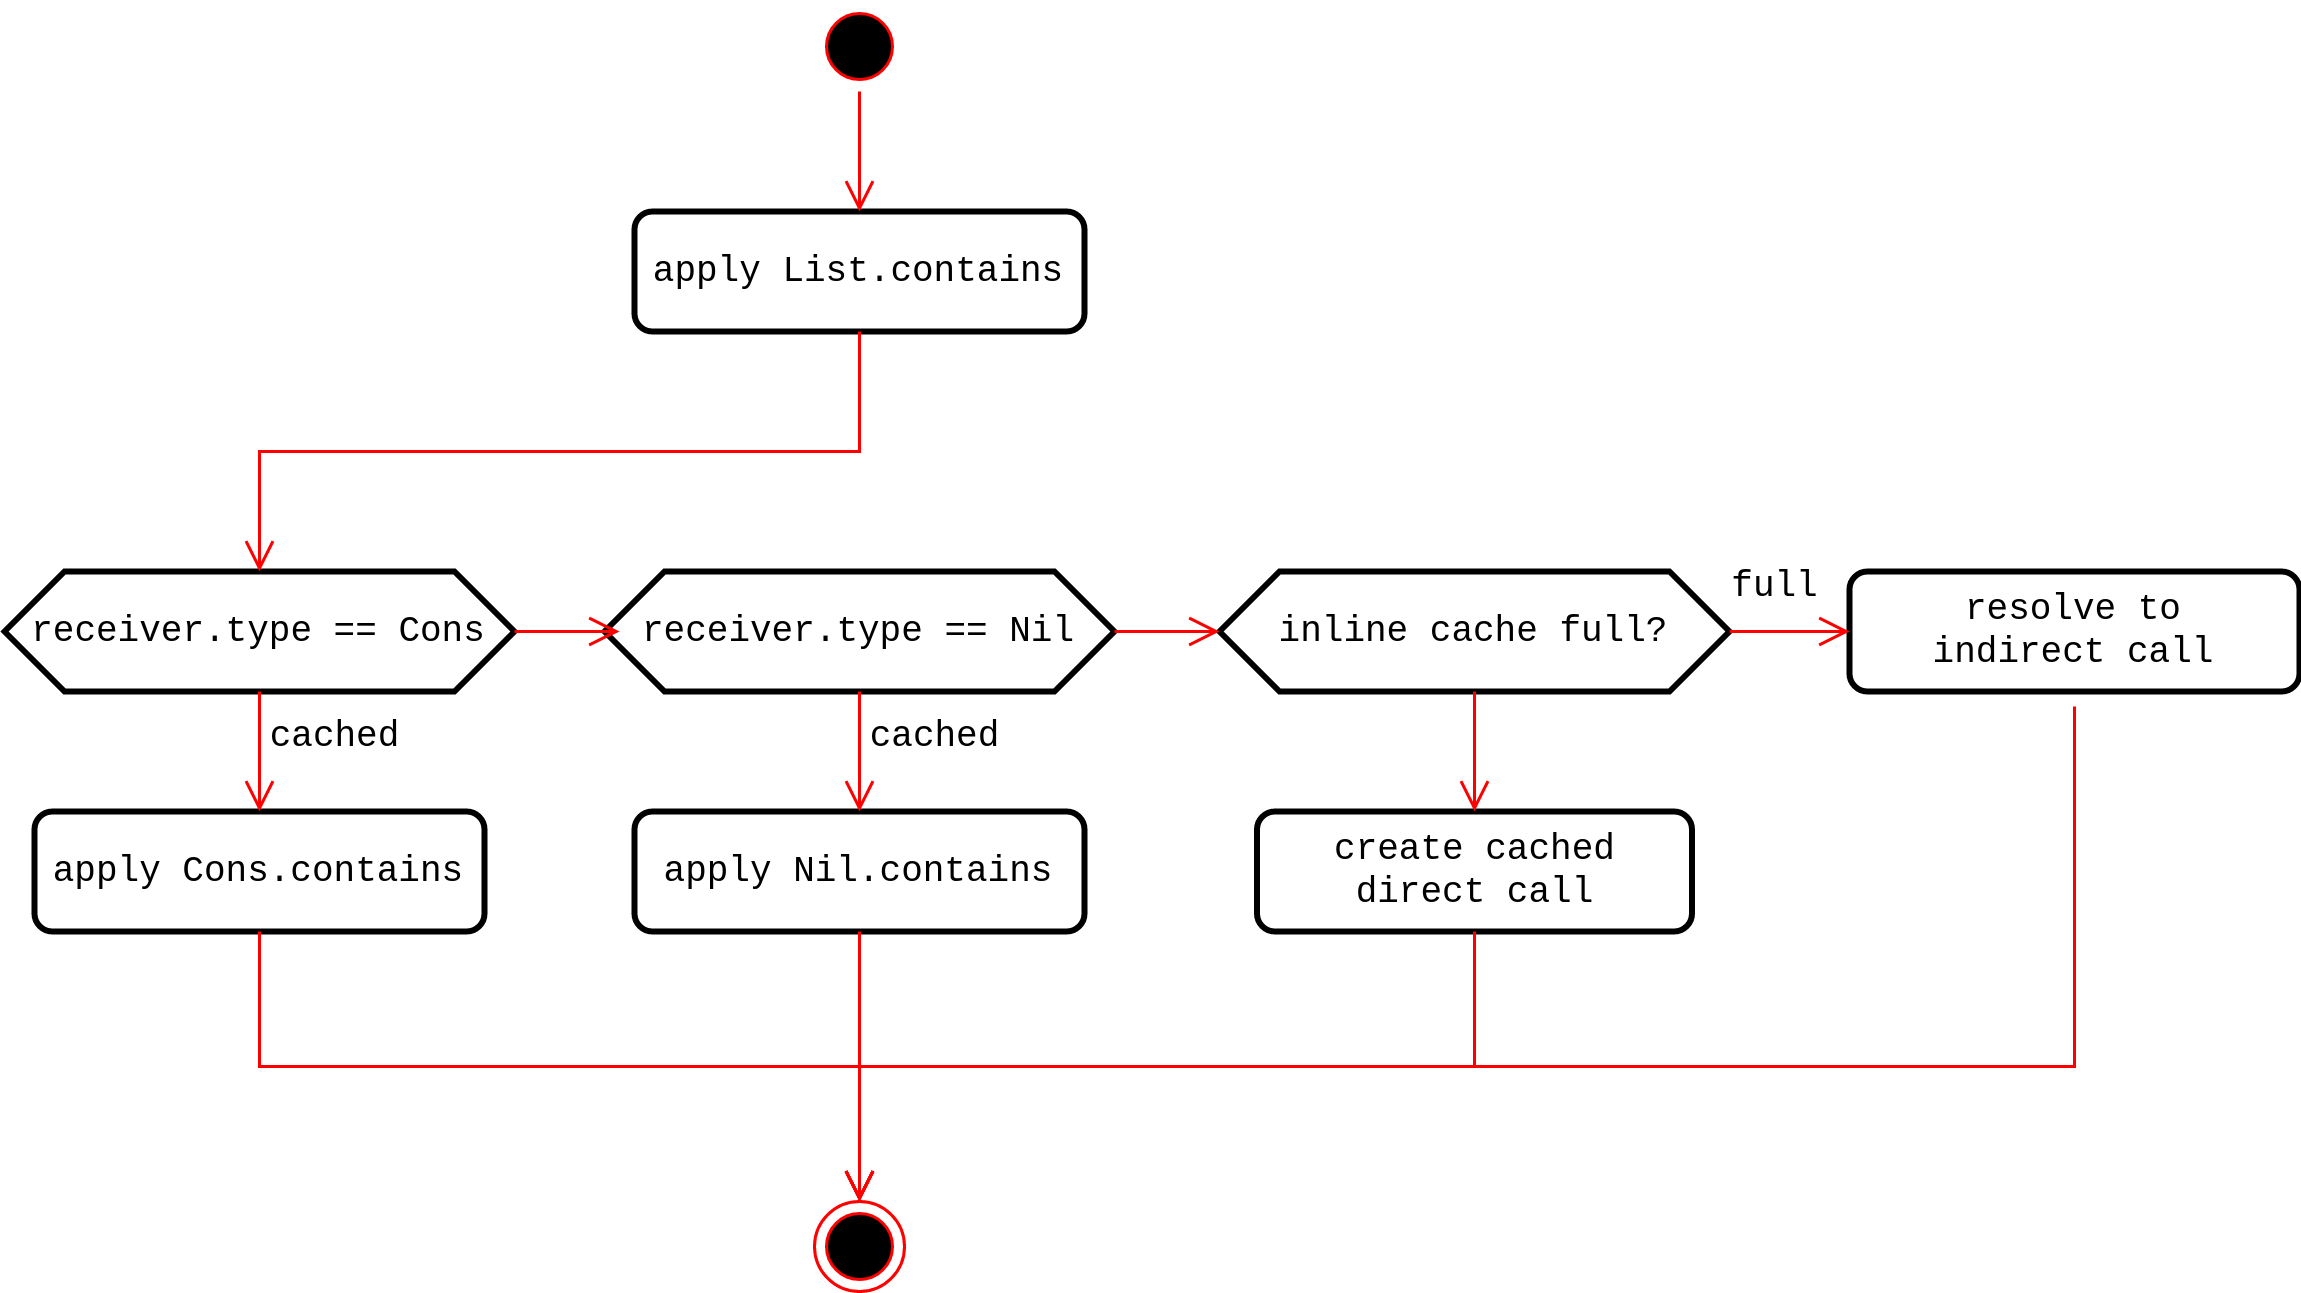
\includegraphics[width=0.6\textwidth]{figures/tastytruffle-pic-example.png}
	\caption{A possible polymorphic inline cache for a \scalainline{List.contains} callsite.}
	\label{example:poly-cache-call-node}
\end{figure}

Figure \ref{example:poly-cache-call-node} shows a data flow diagram of the application of a polymorphic inline cache to a call site of \scalainline{contains} when the receiver type is statically known to be \scalainline{List}. 
The diagram shows that the call site was previously called with a receiver where the dynamic type has been both \scalainline{Cons} and \scalainline{Nil}.
The \scalainline{ApplyNode} will first check if the type of receiver at the call site has the type \scalainline{Cons}; If the check passes, then the cached direct call node is invoked, and the call is complete.
It will do the same for the type \scalainline{Nil}.
Otherwise, the type of receiver has not been seen before, and the call target is resolved virtually and then cached for the following invocation at this call site.

When the polymorphic inline cache is applied to a monomorphic call site (where the type of the receiver does not change), it simplifies to a single element inline cache\cite{smalltalk:inline-caches}. 
Because the type of the receiver at the call site remains stable, the cache look-up of the call target based on the type always succeeds, and the call site never fall backs to using an indirect call node.

\subsection{Accessing Fields}

In our subset of TASTy, the \scalainline{Select} tree represents a read of a field of a \scalainline{ClassInstance}.
Notice in the resolution of the \scalainline{Apply} tree that the \scalainline{Apply} tree represents a method invocation, when the applicator is a \scalainline{Select}.
Because functions are first-class objects in Scala, the TASTy tree for a method invocation is the access of a method as if it were a field, then the application of result to a list of arguments.
Since this case has been previously handled when parsing the \scalainline{Apply} tree, a \scalainline{Select} tree always selects a value definition.

\begin{figure}[!htb]
\begin{minted}{scala}
@NodeChild("receiver")
@NodeField("symbol", Symbol.class)
abstract class ReadFieldNode extends TermNode {
	final val INLINE_CACHE_SIZE: Int = 3;
		
	@Specialization(guards = "instance.getShape == shape", limit = "INLINE_CACHE_SIZE")
	def cached(
		instance: ClassInstance,
		@Cached("instance.getShape") shape: ClassShape,
		@Cached("lookupField(shape)") field: Field
	): Object = field.getContents(instance)
		
	@Specialization(replaces = "cached")
	def virtual(instance: ClassInstance): Object = {
		val field = lookupField(instance.getShape)
		field.getContents(instance)
	}

	private def lookupField(shape: ClassShape): Field = shape.getField(symbol)
}
\end{minted}
\caption{Pseudocode of field read node with a polymorphic inline cache.}
\label{impl:field-read-node}
\end{figure}

\newpage 

However, fields may only be directly accessed in the immediate class scope.
Field access from an outside context is achieved through an \scalainline{accessor}.
Accessors are special methods generated in the compilation pipeline solely to access a field because the Scala compiler enforces the \textit{uniform access principle}\cite{beyer:oo-construction} for all programs.
We apply the transformation to generate accessors in class definitions because accessors are normally generated after TASTy is emitted in the standard Scala compilation pipeline.
Accessors also conveniently provide a mechanism to resolve indirect field access.
Indirect field access occurs when an inherited field is accessed in a subclass.
As we already have a mechanism for resolving method applications, we will combine this mechanism with a new direct field read node to implement field access.

Figure \ref{impl:field-read-node} gives a simplified implementation of a field read node.
Like the virtual dispatch of call targets, fields are resolved dynamically with the shape of a \scalainline{ClassInstance}.
We apply a polymorphic inline cache to the lookup of field properties to eliminate the performance overhead associated with this kind of virtual dispatch.

\subsection{Accessing Locals and Globals}

\begin{figure}[!htb]
\begin{minted}{scala}
def parse(ident: Ident): TermNode = {
	if (ident.symbol.isObjectDef)
		new ReadGlobalNode(symbol)
	else 
		new ReadLocalNode(localOf(symbol))
}
\end{minted}
\caption{Pseudocode to parse an \scalainline{Ident} tree.}
\label{impl:parse-ident}
\end{figure}

The \scalainline{Ident} tree is a name that refers to either a local or global value.
Local values take the form of a local variable or a method parameter.
Global values refer to top-level \scalainline{object} definitions.
We differentiate between a local and a global based on whether the symbol of the \scalainline{Ident} tree refers to a singleton top-level \scalainline{object} definition (shown in figure \ref{impl:parse-ident}).

\begin{figure}[!htb]
\begin{minted}{scala}
object Globals {
	val values: Map[Symbol, ClassInstance]
}

class ReadGlobalNode(symbol: Symbol) extends TermNode {
	override def execute(frame: VirtualFrame): Object = Globals.values.get(symbol)
}

class ReadLocalNode(local: Local) extends TermNode {
	override def execute(frame: VirtualFrame): Object = frame.getObject(local.index)
}
\end{minted}
\caption{Pseudocode of local and global value read nodes.}
\label{impl:local-global-node}
\end{figure}

Figure \ref{impl:local-global-node} provides the pseudocode of \scalainline{ReadGlobalNode} and \scalainline{ReadLocalNode}.
In our interpreter, local variables and method parameters are uniformly represented by the frame slot abstraction.
During parsing, it is sufficient to maintain a mapping from symbols to a \scalainline{Local} to resolve which local variable is read.
Truffle does not provide an abstraction for storing global values.
Instead, we retain a mapping of symbols to instances for all global object value definitions.
Recall from figure \ref{impl:top-level} that a top-level value definition is registered.
When the symbol of an \scalainline{Ident} refers to a \scalainline{ObjectDef}, or a top-level \scalainline{ValDef}, it is resolved using the symbol to look up top-level global values previously registered in \ref{impl:top-level}.

\subsection{Mutating Values}

\begin{figure}[!htb]
\begin{minted}{scala}
def parseAssign(assign: Assign): TermNode = assign match {
	case Assign(select: Select, rhs) => 
		new WriteFieldNode(parse(select.qualifier), select.symbol, parse(rhs)) 
	case Assign(ident: Ident, rhs) =>
		new WriteLocalNode(localOf(ident.symbol), parse(rhs)) 
}
\end{minted}
\caption{Pseudocode to parse an \scalainline{Assign} tree.}
\label{impl:parse-assign}
\end{figure}

The \scalainline{Assign} tree has context-dependent semantics based on the structure of its left-hand side term.
Figure \ref{impl:parse-assign} contains the simplified logic to resolve \scalainline{Assign} trees into the appropriate term nodes.
If the left-hand side term is a \scalainline{Select} tree, the current tree mutates the field of a \scalainline{ClassInstance}.
Otherwise, the left-hand side is an \scalainline{Ident} which refers to the local variable in the frame.
We differentiate between which node to generate based on the type of the tree seen on the left-hand side.
\scalainline{WriteFieldNode} and \scalainline{WriteLocalNode} mirror their read node counterparts, but instead of reading from their respective locations, they update the value at their locations.
Like field reads, field writes in scopes outside of the class are dispatched through \textit{mutators}.
Mutators serve the same purpose as accessors but carry an argument to update the value of the field.

\subsection{Conditionals}

\begin{figure}[!htb]
\begin{minted}{scala}
def parseIf(i: If): IfNode = {
	new IfNode(parse(i.cond), parse(i.thenp), parse(i.elsep))
}
	
class IfNode(
	@Child cond: TermNode, 
	@Child t: TermNode, 
	@Child f: TermNode) extends TermNode {
	val cp = ConditionProfile.create();
		
	override def execute(frame: VirtualFrame): Object =
		if (cp.profile(cond.executeBoolean(frame)))
			t.execute(frame)
		else 
			f.execute(frame)		
}
\end{minted}
\caption{Pseudocode for parsing an \scalainline{If} into an \scalainline{IfNode}}
\label{impl:if}
\end{figure}

The implementation of conditional control flow in our interpreter is quite simple.
Two execution paths exist for the two possible results from evaluating the condition term; the path taken depends on the boolean after evaluation.
An \scalainline{IfNode} is derived from an \scalainline{If} tree (given in figure \ref{impl:if}), which allows for divergence in program control flow.
The implementation of the TastyTruffle IR mirrors the semantics given by its original TASTy tree.
In order to take advantage of conditional speculative optimization, we add a \javainline{ConditionProfile} onto the result of the condition term.
A condition profile records the likelihood that a branch is either true or false.
Graal then speculatively optimizes the frequently true or false branches of an \scalainline{IfNode} using its condition profile.

\subsection{Loops}

In our subset of TASTy, the \scalainline{While} tree is the only looping construct.
The control flow of the \scalainline{While} tree is quite simple; the body term is executed as long as the condition term holds at the beginning of every iteration.
Truffle provides the \scalainline{LoopNode} abstraction for implementations of guest language loop structures.
The loop node abstraction allows guest languages to take advantage of \textit{On-Stack Replacement}\cite{osr}.
On-stack replacement is a technique that switches control of part of a program running in the interpreter to compiled code while that part is executing.

\begin{figure}[!htb]
\begin{minted}{scala}
def parseWhile(tree: While): WhileNode = {
	new WhileNode(parse(tree.cond), parse(tree.body))	
}
	
class WhileNode(@Child cond: TermNode, @Child body: TermNode) extends TermNode {
	
	@Child val loopNode: LoopNode = 
		Truffle.getRuntime.createLoopNode(new WhileRepeatingNode(cond, body))
	
	override def execute(frame: VirtualFrame): Object = {
		loopNode.execute(frame)
		()
	}
	
	class WhileRepeatingNode(
		@Child cond: TermNode, 
		@Child body: TermNode
	) extends Node with RepeatingNode {
		val cp = ConditionProfile.create()
		
		override def executeRepeating(frame: VirtualFrame): Boolean = 
			if (cp.profile(cond.executeBoolean(frame))) {
				body.execute(frame)
				true 
			} else false 
			
	}
}
\end{minted}
\caption{Pseudocode for a \scalainline{WhileNode}}
\label{impl:while}
\end{figure}

So far in this thesis, the root node has been the primary compilation unit in Graal.
Root nodes profile their invocation count and get JIT compiled when they have been invoked frequently.
However, loop constructs that are executed for many iterations also justify JIT compilation.
The loop node is an additional type of JIT compilation unit which Graal can compile.
A key difference between loop nodes and root nodes is when their compiled equivalents are utilized.
While compiled root nodes are used in subsequent invocations of their call targets after they are JIT compiled, compiled loop nodes are used in the next iteration after they are JIT compiled.
As on-stack replacement is not a central focus of this thesis, we will only discuss it briefly, because loop nodes are the recommended abstraction for guest languages to implement loop structures in Truffle.

Figure \ref{impl:while} contains the implementation of a \scalainline{WhileNode} and its derivation from a \scalainline{While} tree.
Like our implementation of the \scalainline{IfNode}, we add a condition profile onto the node which evaluates the termination condition inside \scalainline{WhileRepeatingNode}.
Truffle will automatically instrument the \scalainline{WhileNode}.
After sufficient iterations of the \scalainline{WhileRepeatingNode}, the repeating node is compiled, and the next iteration of the \scalainline{WhileNode} will use the compiled repeating node.

\subsection{Blocks}

\begin{figure}[!htb]
\begin{minted}{scala}
def parseBlock(block: Block): BlockNode = {
	val desc = getParentFrameDescriptor(block)
		
	val terms = block.statements map {
		case vdef: ValDef => generateBlockLocal(desc, vdef)
		case term => term 
	}
		
	new BlockNode(terms, parse(block.expr))
}
	
def generateBlockLocal(desc: FrameDescriptor, vdef: ValDef): TermNode = {
	val local = generateLocal(vdef)
	new WriteLocalNode(local, parse(vdef.rhs))
}	
\end{minted}
\caption{Pseudocode for parsing \scalainline{Block} into \scalainline{BlockNode}}
\label{impl:parse-block}
\end{figure}

This section covers the translation of the \scalainline{Block} tree to its TastyTruffle IR equivalent.
The \scalainline{Block} is unique among term trees as it describes data and code.
In our subset of TASTy, this means that a block may contain declarations of local variables as well as executable terms.
Figure \ref{impl:parse-block} provides an overview on the transformations necessary to convert a \scalainline{Block} tree into \scalainline{BlockNode}.
We divide the discussion of blocks into the resolution of local variables when encountering a \scalainline{ValDef} tree and the execution of all other trees.

Local variables are bound to a \textit{scope}. 
A scope represents the lifetime in which a variable can refer to a value. 
Similarly, uses of variables are only valid when used under the appropriate scope. 
Local variables and their use sites are represented in intermediate representations through various methods. 
In abstract syntax trees, local variables and their uses are represented as nodes \textit{dominated} by their scopes (which are themselves nodes). 
In our subset of TASTy, a \scalainline{ValDef} dominated by a \scalainline{Block} represents a local variable.
When a \scalainline{ValDef} tree is present in this context, the right-hand side of the value definition will be non-empty.
A local variable declaration in Scala must always be accompanied with an initial value.

\begin{figure}[!htb]
\begin{minted}{scala}
class BlockNode(stats: Array[TermNode], last: TermNode) extends TermNode {
	@ExplodeLoop
	override def execute(frame: VirtualFrame): Object = {
		for (stat <- stats) 
			stat.execute(frame)
		last.execute(frame)
	}
}
\end{minted}
\caption{Pseudocode of the \scalainline{BlockNode}}
\label{impl:block-node}
\end{figure}

Because terms always return a value, the \scalainline{Block} tree must follow the same semantics.
Figure \ref{impl:block-node} gives the pseudocode for our implementation of a \scalainline{BlockNode}.
The \javainline{@ExplodeLoop} is a Truffle DSL directive that guides Graal to unroll\cite{loop-unrolling} the loop for the execution of each child node.
Unrolled loops simplify partial evaluation as each iteration of the loop is treated as an individual statement, and thus they reveal constant values, which are simpler for partial evaluation.
As the number of children in a \scalainline{BlockNode} is known before execution, it makes sense to unroll the loop to simplify optimization.
\newpage
\subsection{Returns}

\begin{figure}[!htb]
\begin{minted}{scala}
class ReturnException(result: Object) extends ControlFlowException

class ReturnNode(@Child term: TermNode) extends TermNode {
	override def execute(frame: VirtualFrame): Object = { 
		val result = term.execute(frame)
		throw new ReturnException(result)
	}
}
\end{minted}
\caption{Pseudocode of \scalainline{ReturnException} and \scalainline{ReturnNode}}
\label{impl:return}
\end{figure}

A \scalainline{Return} tree ends the execution of the current method and passes a value back to the caller.
The semantics of returning control flow in Truffle is implemented as a program \textit{exception}.
An exception is an unexpected disruption of program control flow.

The implementation of the \scalainline{ReturnException} and \scalainline{ReturnNode} is given in figure \ref{impl:return}.
The \scalainline{ReturnException} is a subclass of the \javainline{ControlFlowException}. 
Control flow exceptions are special exceptions that Truffle treats differently from other JVM exceptions for control flow analysis.
A return exception is thrown with the return value evaluated from a return node.
The exception is then caught by the executing \scalainline{DefDefNode}, where the return value is passed back to the caller. 

Recall in figure \ref{impl:defdefnode} that a body of a \scalainline{DefDefNode} is executed and a \scalainline{ReturnException} is possibly caught.
If a \scalainline{ReturnException} is not caught, the callee did not encounter a \scalainline{ReturnNode} during its execution.
By default, Scala methods always return the result computed by the last term in the outermost block of a method if no other \scalainline{return} expressions are present in the control flow of the method. 

\subsection{Putting it All Together}

\begin{figure}[!htb]
\begin{minted}{scala}
Block(
	ValDef("these", _, This),			
	While(
		Apply(Select(Ident("these"), "empty"), "!", List.empty),
		If(
			Apply(
				Select(Select(Ident("these"), "head"), "=="), 
				Ident("elem")
			),
			Return(Constant(true)),
			Assign(Ident("these"), Select(Ident("these"), "tail"))
		)	
	),
	Constant(false)
)
\end{minted}
\caption{TASTy of \scalainline{Cons.contains}}
\label{tasty:list-contains}
\end{figure}

In this section, we summarize all the tree transformations introduced for the monomorphic variant of our interpreter.
Figure \ref{tasty:list-contains} is the structure of the \scalainline{Cons.contains} method in TASTy.
We have omitted the type tree, which has been declared inside the local variable definition.
We use the \scalainline{Cons.contains} method as an example to summarize the transformations described in this section.

\begin{figure}[!htb]
\begin{minted}{scala}
BlockNode(
	WriteLocalNode("these", ReadLocalNode("this")),
	WhileNode(
		UnaryOpNode("!",  ApplyNode("these", "List.isEmpty[0]()", Array.empty)),
		IfNode(
			ApplyNode(
				FieldReadNode(ReadLocalNode("these"), "head"), 
				"Any.==[0]()", 
				ReadLocalNode("elem")
			),
			ReturnNode(ConstantNode(true)),
			WriteLocalNode("these",  ReadFieldNode(ReadLocalNode("these"), "tail")),	
		)   
	),
	ConstantNode(false)
)
\end{minted}
\caption{\scalainline{Cons.contains} as a Truffle AST}
\label{example:truffle-list-contains}
\end{figure}

Figure \ref{example:truffle-list-contains} is the Truffle equivalent AST of \scalainline{Cons.contains}.
Simple strings are used to represent symbols and method signatures to avoid unnecessary detail in the example.
Notice that many TASTy nodes have an equivalent TastyTruffle IR, which closely mirrors their structure.
However, other TASTy nodes must be simplified to a representation more suitable for runtime.
In particular, \scalainline{ValDef} trees are eliminated and replaced by an initializer node that assumes the frame slot for the local variable definition was added during parsing.
In chapter \ref{implementation:specialization}, the challenges of using these trees in the presence of parametric polymorphism and their associated performance overhead will be described.

\chapter{The Polymorphic Interpreter}
\label{implementation:specialization}

\begin{figure}[!htb]
\begin{minted}{scala}
abstract class TypeNode extends Term {
	override final def execute(frame: VirtualFrame): Object = resolveType(frame)
	def resolveType(frame: VirtualFrame): Type 
}
\end{minted}
\caption{An abstract type node.}
\label{impl:type-node}
\end{figure}

In this chapter, The interpreter will be extended to support the execution of polymorphic trees.
To that end, the notion of \textit{reified} type nodes will be introduced.
In essence, to implement specialization of polymorphic classes and methods, types will be treated as \textit{first-class} values.
Like the \scalainline{TermNode} represents the \scalainline{Term} tree node from TASTy, the \scalainline{TypeNode} represents the \scalainline{Type} from TASTy but instead of producing a value from evaluation, it produces a \textit{type}.
To better illustrate this concept, figure \ref{impl:type-node} contains the implementation of the node superclass that evaluates to a type and not a value.

\begin{figure}[!htb]
\begin{minted}{scala}
parseType(tpe: Type): TypeNode = tpe match {
	case ref: TypeRef => TypeRefNode(ref)
}

class TypeRefNode(ref: TypeRef) extends TypeNode {
	override def resolveType(frame: Frame): Type = ref
}
\end{minted}
\caption{A \scalainline{TypeNode} for handling type references.}
\label{impl:parse-type}
\end{figure}

Figure \ref{impl:parse-type} gives the simplified implementation to reify type references in the polymorphic interpreter.
For now, we will limit the scope of reified type to the simplest and introduce concepts that integrate reified types with Truffle abstractions further in the chapter.
Figure \ref{impl:extend-new} extends the \scalainline{NewNode} to support the creation of object instances using reified type nodes.
Because a type reference essentially reifies statically available type information, very little changes in the implementation of a \scalainline{NewNode}.

\begin{figure}[!htb]
\begin{minted}{scala}
def parseNew(new: New): NewNode = new NewNode(parseType(new.tpe))	

class NewNode(@Child typeNode: TypeNode) extends TermNode {
	override def execute(frame: VirtualFrame): Object = {
		val tpe = typeNode.resolveType(frame)
		shapeOf(tpe).newInstance
	}
}
\end{minted}
\caption{Extension to the \scalainline{NewNode} for the polymorphic interpreter.}
\label{impl:extend-new}
\end{figure}

Because types are erased from their instantiation sites in Java bytecode, the underlying type of a type parameter are not normally known during runtime. 
Introducing types during execution will allow data layouts to be determined at runtime.
The type node is the abstraction we use to encapsulate this concept.
The principal idea behind the type node is to allow for the resolution of types during runtime.
Introducing a mechanism to resolve types during runtime avoids the pitfalls of type erasure.
In this half of the chapter, whenever we discuss the advantages of the polymorphic interpreter, we will use a monomorphic interpreter where the code has undergone type erasure as our frame of reference.

Using the newly available type information during runtime, data layout can be specialized based on the types seen.
In the following subsections, we will focus on specific instances of boxing using Graal IR for compiled code executed using the monomorphic interpreter.
Then we introduce subclasses of the \scalainline{TypeNode} and show how reified types can be utilized to specialize the data layouts from the monomorphic interpreter.

\section{Specializing Methods}

\begin{figure}[!htb]
\begin{minted}{scala}
class DefDefTemplate(
	desc:    FrameDescriptor
	tparams: Int, 
	vparams: List[ValDef | LocalFrameVal], 
	locals:  List[ValDef | LocalFrameVal],
	rhs:     Term
) extends RootNode(desc) {
	def execute(frame: VirtualFrame): Object = ???
	def specialize(types: Array[Type]): DefDefNode = ???
}
\end{minted}
\caption{Pseudocode for a \scalainline{DefDefTemplate}.}
\label{impl:defdeftemplate}
\end{figure}

Polymorphic methods in Scala can be polymorphic under class type parameters, method type parameters, or both (see \ref{example:cons-impl}). 
This section will focus only on the specialization of polymorphic methods under their type parameters.
We defer the discussion of the specialization of class-polymorphic methods until the next section.
We will introduce the concept of a \textit{template}; templates retain sufficient information about the data layout of a definition in TASTy to generate their runtime representations dynamically.
Instead of a \scalainline{DefDefNode}, a \scalainline{DefDefTemplate} (given in figure \ref{impl:defdeftemplate}) is a root node that represents a polymorphic method. 
When a \scalainline{DefDefTemplate} is specialized, the result is a monomorphic \scalainline{DefDefNode} specialization.
As Truffle does not have mechanisms that support root node rewriting at the current time, we describe how to use Truffle DSL constructs to make method specialization performant.

\begin{figure}[!htb]
\begin{minted}{scala}
def parseDefDef(ddef: DefDef): DefDefNode | DefDefTemplate = {		
	val tparams = ddef.params.filter(_.isInstanceOf[TypeDef]).length
	if (tparams == 0)
		createDefDefNode(ddef)
	else {
		val vparams = ddef.filter(_.isInstanceOf[ValDef]) map {
			case vdef @ ValDef(_, tpt, rhs) => 
				if (tpt.tpe.isTypeParameter) 
					vdef
				else
					generateLocal(vdef)
		}
	
		val locals = liftLocals(ddef.rhs)
		new DefDefTemplate(desc, tparams, vparams, locals, ddef.rhs)
	}
}

def createDefDefNode(ddef: DefDef): DefDefNode // a monomorphic DefDef
	
...
\end{minted}
\caption{Pseudocode for parsing \scalainline{DefDef} into \scalainline{DefDefNode}}
\label{impl:parse-poly-defdef}
\end{figure}

The specialization of a \scalainline{DefDefTemplate} begins at invocation.
Because type arguments are introduced at specific polymorphic call sites, method specializations must be created at or after invocation.
When a method template is invoked with both type and value arguments, it forwards the value arguments to the appropriate specialization based on the type arguments.

The specialization of a method template is the ad hoc creation of a root node with a specialized frame descriptor.
A \scalainline{DefDefTemplate} retains the number of type parameters it owns; this is sufficient to resolve type arguments for creation and dispatching to specializations, and type parameters never collide by name.
Source information about value parameters is stored on a template instead of abstracted local frame values.
The type of value parameter can potentially be resolved from a method type parameter.
Since the frame descriptor is unpopulated because value parameters are possibly polymorphic, it is not yet appropriate to create executable term nodes that may read from or write to the frame slots of polymorphic value parameters.
Figure \ref{impl:parse-poly-defdef} extends the transformation of a \scalainline{DefDef} to include method templates.

\subsection{Invoking Polymorphic Methods}

\begin{figure}[!htb]
\begin{minted}{scala}
def parseApply(apply: Apply): ApplyNode = {
	val signature = apply.symbol.signature
	apply match {
		case Apply(Select(qualfier, _), arguments) => ... // monomorphic trees
		case Apply(TypeApply(Select(qualifier, _), targs), args) =>
			new ApplyNode(signature, parse(qualifier), (targs ++ args).map(parse))
	}
}
\end{minted}
\caption{Extension to parsing a polymorphic \scalainline{Apply} tree.}
\label{impl:parse-typeapply}
\end{figure}

In this section, we demonstrate when and where polymorphic methods are invoked.
For this demonstration, we will show one of the natural benefits of executing TASTy.
A polymorphic method invocation in TASTy is always an \scalainline{Apply} tree node where the qualifier is a \scalainline{TypeApply}.
The \scalainline{TypeApply} tree node represents a \textit{type application}.
Without delving into great detail, a type application is the process of producing a monomorphic method from a polymorphic method by unification.
Analogous to normal applications, which accept values as arguments and produce values as results, type applications accept types as arguments and produce values as a result.
With this in mind, \scalainline{TypeApply} nodes are a naturally suitable site to invoke and create specializations for methods.

\begin{figure}[!htb]
\begin{minted}{scala}
def apply(T: Type, array: Array[T]): List[T] = T match {
	case Int => apply$Int(array.asInstanceOf[Array[Int]])
	...
	case _   => apply$Any(array.asInstanceOf[Array[Any]])
}
\end{minted}
\caption{Pseudocode that mimics the implementation of specialized method dispatch using Scala sources.}
\end{figure}

Figure \ref{impl:parse-typeapply} extends the transformation of \scalainline{Apply} tree nodes to include polymorphic applications.
The application of a polymorphic method follows the same semantics as the application of a monomorphic method.
The actual specialization of the frame layout occurs inside the template that a polymorphic \scalainline{ApplyNode} invokes.
This design decision allows the invocation of polymorphic methods even in the presence of dynamic dispatch.
In the next section, we will describe the additional machinery that is added \textit{after} a polymorphic inline cache has resolved virtual dispatch to handle type application and how to make such mechanisms amenable for partial evaluation.

\newpage
\subsection{Typed Dispatch Chains}

\begin{figure}[!htb]
\begin{minted}{scala}
class DefDefTemplate(...) extends RootNode(...) { 
		
	@CompilerDirectives.CompilationFinal
	val specializations: Array[(Array[Type], DirectCallNode)] = Array.empty
		
	def execute(frame: VirtualFrame): Object = {
		val typeArgs = resolveArguments
		dispatchCached(frame, typeArgs)
	}
		
	@ExplodeLoop
	def dispatchCached(frame: VirtualFrame, typeArgs: Array[Type]): Object = {
		for ((typeSig, specialization) <- specializations)
			if (typeSig == typeArgs)
				return specialization.call(frame.getArguments)
		CompilerDirectives.transferToInterpreterAndInvalidate()
		dispatchNew(frame, typeArgs)
	}
	
	def dispatchNew(frame: VirtualFrame, typeArgs: Array[Type]): Object = {
		val specialization = specialize(typeArgs)
		val callNode = DirectCallNode.create(specialization)
		specializations += (typeArgs -> callNode)
		callNode.call(frame.getArgs)
	}
	
	...
}
\end{minted}
\caption{Pseudocode for typed dispatch inside a \scalainline{DefDefTemplate}.}
\label{impl:defdeftemplate-execute}
\end{figure}

Dispatch chains\cite{trufflyruby:specialization} are multi-layered inline caches.
We introduce the notion of \textit{typed dispatch chains}.
Typed dispatch chains integrate the semantics of type applications via a second inline cache after virtual call resolution.
Figure \ref{impl:defdeftemplate-execute} contains the simplified implementation of the execution semantics in a \scalainline{DefDefTemplate}.

Specializations of polymorphic methods are created on demand and then cached based on their reified type signatures.
One challenge of making caching mechanisms fold away in partial evaluation is that the cache must be a \textit{compilation constant}.
Type arguments at type application sites are always stable, i.e., their respective type nodes evaluate to the same type; the look-up of the specialized call node should have no overhead when JIT compiled with the aid of partial evaluation. 
We exploit a simple array of type signatures and specialized call node pairs to make this possible.
When the loop for looking up a cache entry in the array is unrolled during partial evaluation (directed by \javainline{ExplodeLoop}), the loop is transformed into a block of conditional expressions for each cache entry.
This unrolled loop, combined with the injected knowledge that type argument values are compilation constants, results in the conditional elimination\cite{conditional-elim} of checks for non-matching cache entries.
Once the appropriate specialization is found, the call is forwarded to the root node, which contains the specialized term nodes.

When a combination of type arguments has not yet been encountered and their corresponding specialization is unavailable, the specialization must be generated and invoked.
To prevent this \textit{slow} path of execution from being JIT compiled, we direct the compiler to \textit{bail out} of JIT compilation with the \scalainline{transferToInterpreterAndInvalidate} directive.
The directive allows guest languages to insert their own deoptimization points into the control flow of a program; this ensures code of the slow branch when creating the specialization is never compiled.
Note that in the first case where a type argument lookup succeeds (the fast path), the directive is unreachable because the control flow of the code returns and, therefore, will not be part of compiled code.

\begin{figure}[!htb]
	\centering
	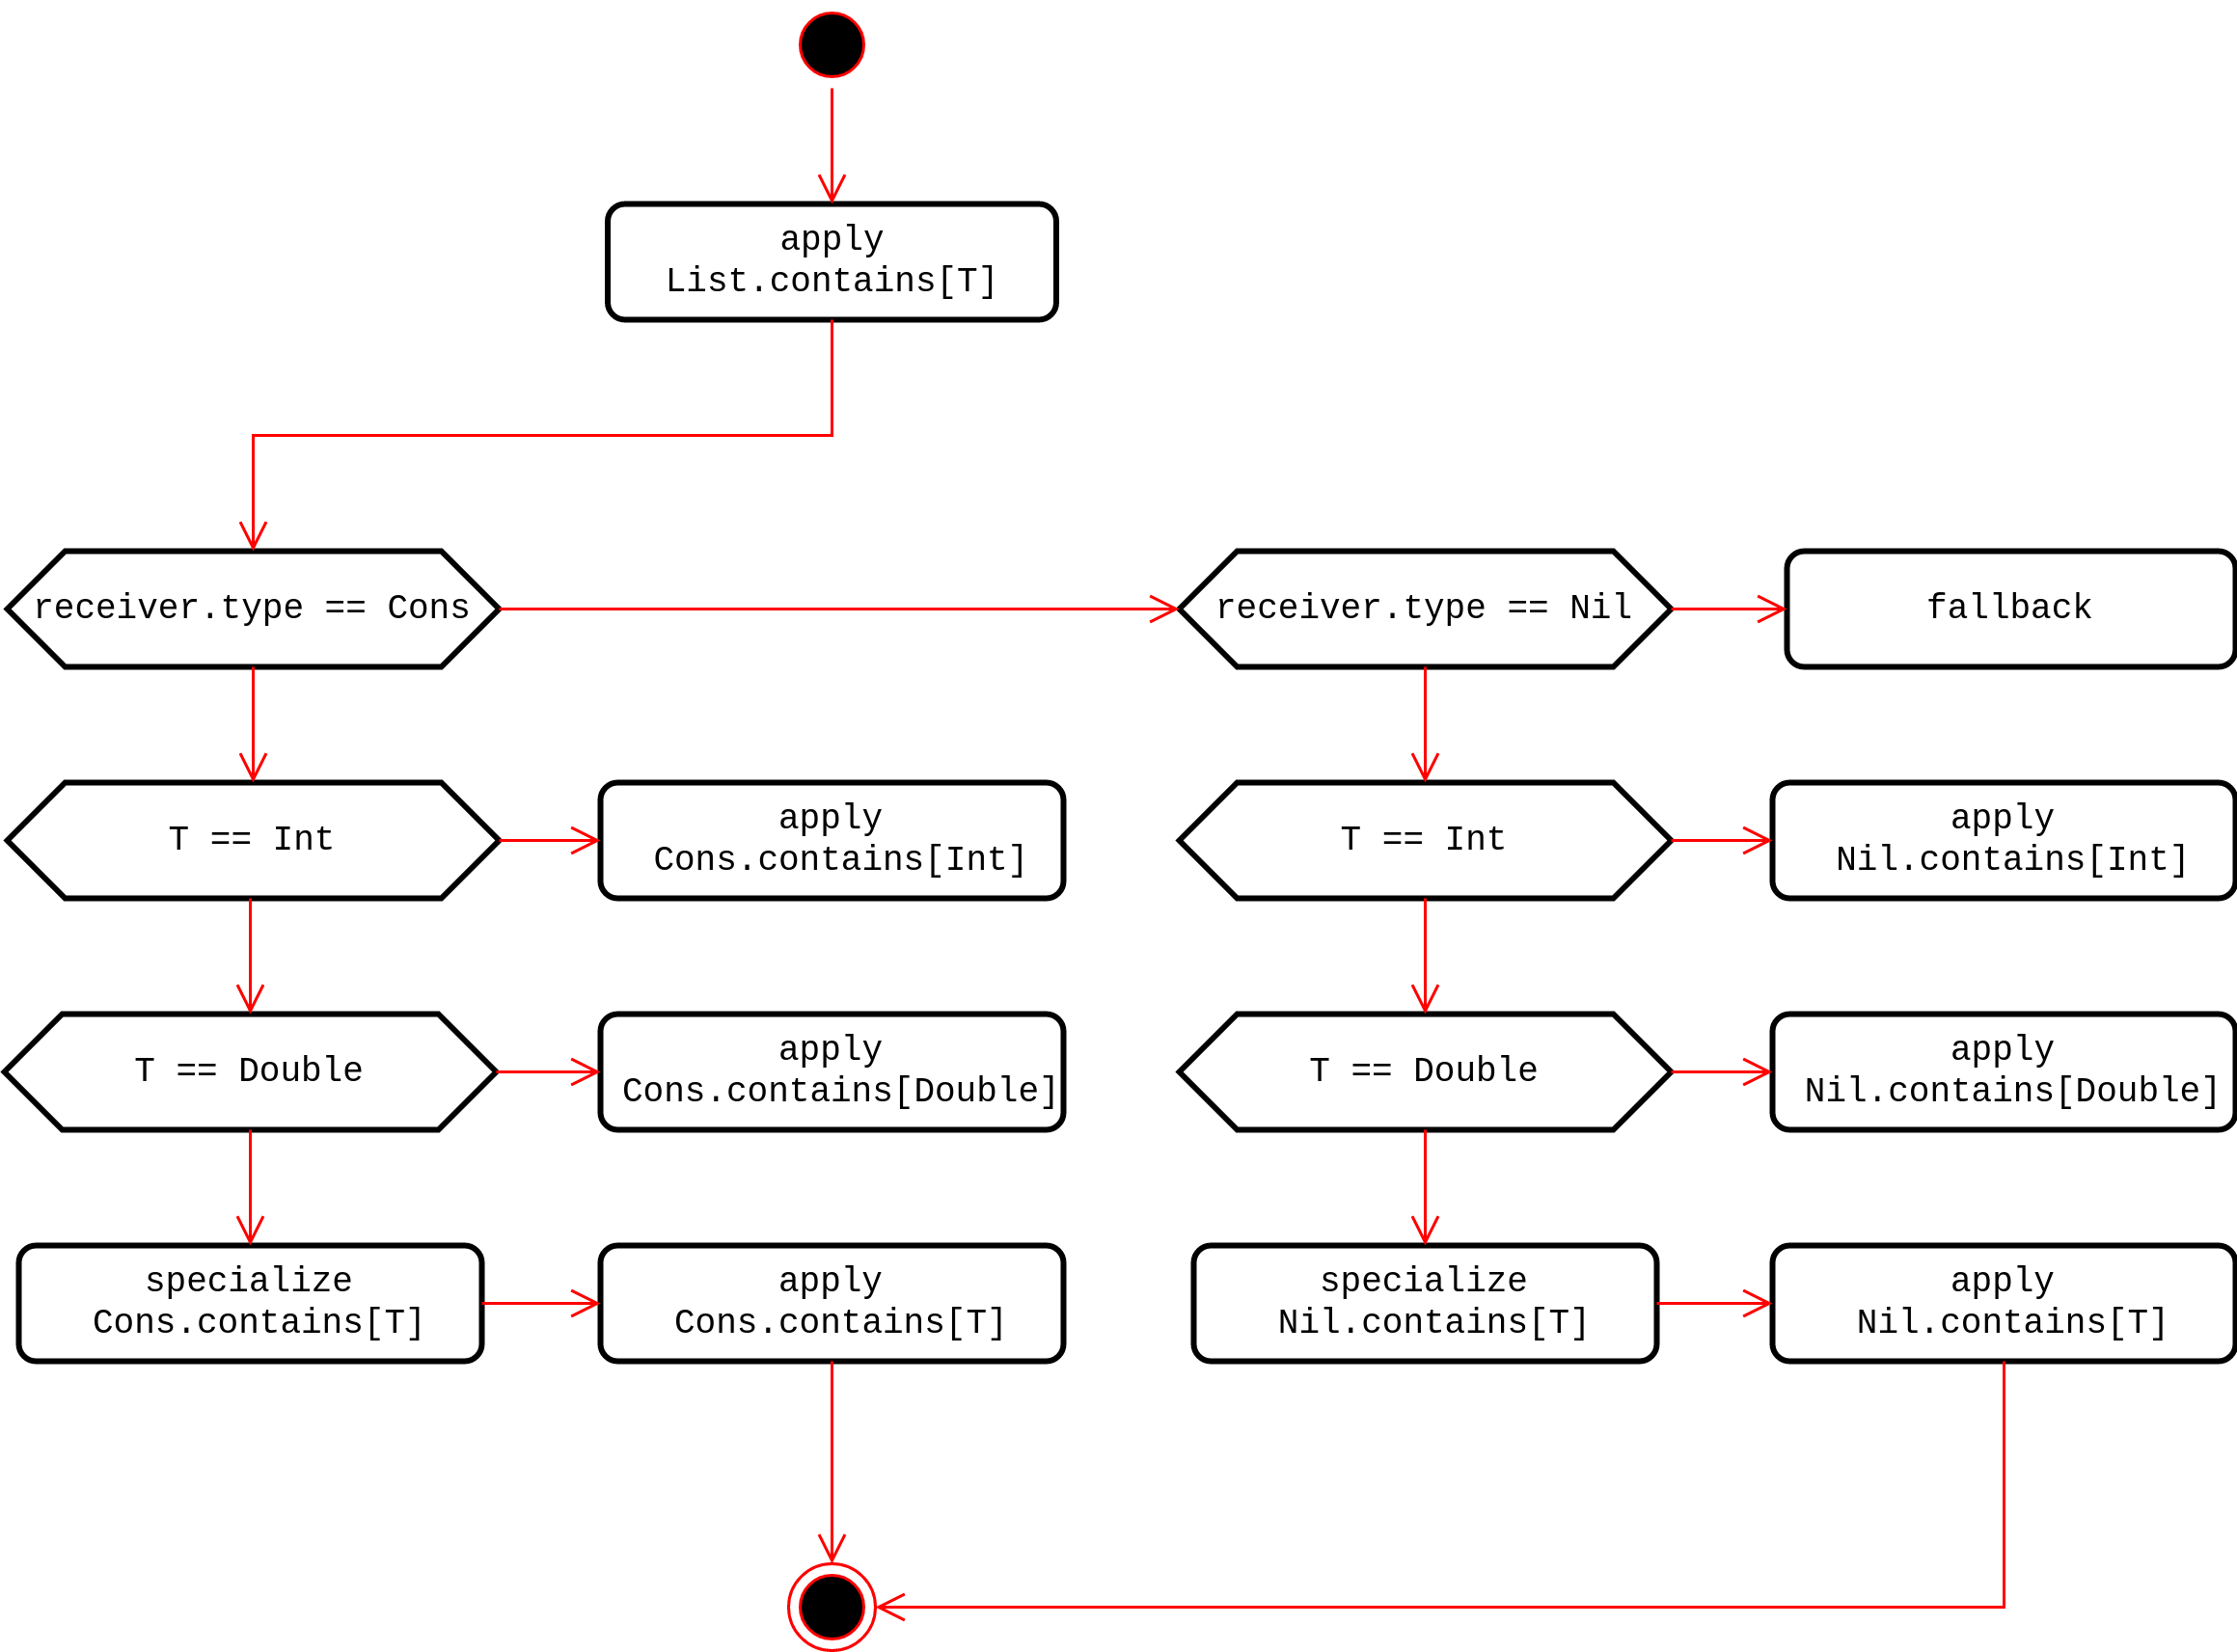
\includegraphics[width=0.75\textwidth]{figures/tastytruffle-type-dispatch-chain.png}
	\caption{The typed dispatch chain for a \scalainline{List.contains} call site}
	\label{example:typed-dispatch}
\end{figure}

Figure \ref{example:typed-dispatch} is an extension of the example given in figure \ref{example:poly-cache-call-node} with typed dispatch.
The example assumes the type arguments for \scalainline{Int} and \scalainline{Double} for \scalainline{Cons.contains[T]} and \scalainline{Nil.contains[T]} has previously been specialized and cached.
After the polymorphic inline cache resolves the receiver to an exact type, the corresponding specialization is looked up.
While this example may seem deceptively large, only the path taken in the control flow is compiled after partial evaluation.
For example, consider the invocation \scalainline{List.contains[Int]} when the receiver is an instance of \scalainline{Cons}.
The corresponding compiled code will not contain the check that type parameter is an \scalainline{Int}.
Because all other program logic is eliminated during partial evaluation, the inlining of calls is also straightforward.
After the partial evaluation, the typed dispatch mechanism is also eliminated, and the specialized method is the only code remaining.

\subsection{Case Study: The Subset of a List}

Recall the implementation of \scalainline{contains} given in figure \ref{example:cons-impl}.
An implementation of a method using \scalainline{contains} to determine if a list is the subset of another is given in \ref{example:list-subset}.
This case study is implemented for \scalainline{List[Int]} in order to showcase method specialization in the context of control flow without consideration for class specialization.
More specifically, this case study will examine how repeated invocations of \scalainline{Cons.contains[Int]} will interact with the interpreter.

In the initial execution of the \scalainline{subset} method in the interpreter, profiling information about call receiver types and type arguments are collected.
The invocation of \scalainline{contains} during the first iteration of the loop given in line $3$, the virtual call is indirect and the specialization for \scalainline{contains[Int]} does not exist.
First, the call target for the concrete implementation of \scalainline{contains} is resolved and entered into the inline cache.
Second, the specialization for \scalainline{contains[Int]} is created and entered into the inner typed inline cache.

\begin{figure}[!htb]
\begin{minted}{scala}
def subsetInt(fst: List[Int], snd: List[Int]): Boolean = {
	var iter: List[T] = fst
	while (!iter.isEmpty) 
		if (!snd.contains(iter.head))
			return false 
	true
}
\end{minted}
\caption{Implementation of \scalainline{subset}.}
\label{example:list-subset}
\end{figure}

Invocations of \scalainline{contains} in subsequent iterations of the loop where the receiver type is stable, the virtual call is inline and forwarded to the specialization for \scalainline{Int}.
Therefore, the invalidation condition in the JIT compiled variant of the code assumes the type of receiver has not changed.
Because receiver types are dynamic and type arguments are static at call sites, a change in the type of receiver at a call site is is sufficient for invalidation.
If this assumption is violated, execution resumes in the interpreter and profiling information is again collected for a future JIT compilation.

This process repeats for each receiver type seen at a call site and specialization occurs once for each of the call targets that are resolved through virtual dispatch.
Note that for $N$ possible types seen in the receiver at a call site, only $N$ specializations will be created.
The assumption generated by Truffle guard both cache lookup operations in the typed dispatch chain.
By integrating typed dispatch into an inner inline cache after virtual call resolution, no additional assumptions are generated by Truffle for JIT compilation.

\subsection{Specializing Polymorphic Parameters}

The data layout of a method is given by the frame descriptor of its root node.
A specialized method will have a specialized frame descriptor.
Specialized frame descriptors will have the appropriate primitive frame slot kinds assigned to value definitions that have their polymorphic types resolved to a primitive type.
Therefore, the core principle behind method specialization is generating a \scalainline{TermNode} tree from a \scalainline{Term} tree using a specialized frame descriptor.
Apart from extensions given earlier in this section, the parsing of \scalainline{Term} nodes does not differ from their monomorphic counterparts.

Figure \ref{impl:gen-poly-locals} gives an extension to generate frame slots from type parameters and polymorphic value definitions associated with the method to generate frame slots from monomorphic value definitions.
Like its counterpart in the monomorphic interpreter, the abstraction for a local frame value in the polymorphic interpreter has a slot.
However, a local frame value in the polymorphic interpreter retains a type instead of a frame slot kind.
If the type of a value parameter can be resolved with the type arguments supplied during specialization, the specialized frame slot is created and added to the descriptor.

\begin{figure}[!htb]
\begin{minted}{scala}
class DefDefTemplate(...) extends RootNode(...) {
	def execute(frame: VirtualFrame): Object = ...
		
	def specialize(types: Array[Type]): DefDefNode = {
		val desc = this.desc.copy()
			
		val parameters = self :: vparams.map(specializeValDef(types, desc))
		locals.foreach(specializeValDef(types, desc))
			
		val body = parse(rhs)
		new DefDefNode(desc, parameters, body)
	}

	def specializeValDef(
		types: Array[Type], 
		desc:  FrameDescriptor, 
		v:     LocalFrameVal | ValDef
	): LocalFrameVal = v match {
		case vdef: ValDef => generateLocal(types, vdef, desc)
		case v => v
	}
}
\end{minted}
\caption{Pseudocode for on-demand specialization inside a \scalainline{DefDefTemplate}.}
\label{impl:defdeftemplate-specialize}
\end{figure}

$$
index(\tau) = 
\begin{cases}
	i  & \textbf{def } f[t_0, \ldots, t_i, \ldots, t_n](\ldots) \text{ if } t_i = \tau, owner(\tau)=f \\
	-1 & \text{otherwise}
\end{cases}
$$

Figure \ref{impl:defdeftemplate-specialize} contains the pseudocode for creating specialized root nodes and accompanying frames using type arguments.
A mapping of types (via their symbols) to their respective index in the type argument array is sufficient to handle this resolution.
The symbol \textit{owner} is the symbol of the tree that encloses the current tree.
Because we are only discussing methods polymorphic under their own type parameters, all polymorphic value parameters are resolved in this context.
The derivation of local frame values from monomorphic value definitions remains unchanged. 

\begin{figure}[!htb]
\begin{minted}{scala}
def generateLocal(
	types: Array[Type], 
	defn: ValDef | TypeDef, 
	desc: FrameDescriptor): LocalFrameVal = defn match {
		case tdef: TypeDef => 
			val kind = FrameSlotKind.Object
			val slot = desc.addSlot(kind)
			LocalFrameVal(slot, ReifiedType)
		case vdef: ValDef => 
			val idx  = index(vdef.tpt.tpe)
			val tpe  = if (idx != -1) types(idx) else vdef.tpt.tpe
			val kind = getFrameSlotKind(tpe)
			val slot = desc.addSlot(kind)
			LocalFrameVal(slot, tpe)
	}
\end{minted}
\caption{Extension to pseudocode that generates frame slots to include polymorphic definitions.}
\label{impl:gen-poly-locals}
\end{figure}

A type definition is treated in the same manner as a value definition; it is assigned a frame slot with an \javainline{Object} frame slot kind.
This allows storing types in the method frame, allowing for the resolution of types after invoking a method template.
So far, we have only discussed the resolution of type arguments in an intraprocedural context.
Storing reified types in the frame during execution allows for the resolution in an interprocedural context.
We will detail why this is important in the following subsection.

Truffle conveniently profiles the types of frame arguments to speculatively eliminate the unboxing of boxed values when reading frame values (including arguments). 
For example, the following invocation \scalainline{list.contains((elem: Int))} will be profiled by Truffle even if we store \scalainline{elem} in an \scalainline{Object} frame slot.
Truffle will then speculatively unbox \scalainline{elem} in the body of \scalainline{contains} if appropriate.
These optimizations and their limits are discussed in Chapter \ref{chapter:evaluation}.

\begin{figure}[!htb]
\begin{minted}{scala}
def maximum[T <: Numeric](list: List[T]): Boolean =  {
	var max: T  = zero
	var curr: List[T] = a
	while (!curr.isEmpty) 
		if (curr.head > max)
			max = curr.head 
	max
}
\end{minted}
\caption{Implementation of a \texttt{max} method for a \scalainline{List}.}
\label{impl:list-max}
\end{figure}

\newpage 

In contrast, write operations of polymorphic frame values cannot be speculatively eliminated. 
Because Truffle does not specialize data layouts, i.e., frames are determined by their descriptors, which in turn are determined by the guest language implementation, frame writes of polymorphic values will always have to be boxed.
The elimination of boxed polymorphic writes from frame descriptor specialization is one of the major benefits when compared to the monomorphic interpreter.
Code that has polymorphic code, which reads and writes to a frame frequently, will no longer have to unbox, compute primitive operations on unboxed values, then box those values back into their respective slots.
Figure \ref{impl:list-max} contains an example program with polymorphic code that frequently writes to a polymorphic local variable after some computation.

\subsection{Case Study: A List Constructor}

\begin{figure}[!htb]
\begin{minted}{scala}
object List {
	def apply[T](array: Array[T]): List[T] = {
		var i = array.length - 1
		var these: List[T] = Nil
		while (i >= 0) {
			these = new Cons[T](array(i), these)
			i -= 1
		}
		these
	}	
}
\end{minted}
\caption{An alternate static constructor that converts an \scalainline{Array[T]} to a \scalainline{List[T]}}
\label{impl:list-alt-constructor}
\end{figure}

In this section, we examine an example containing code Truffle cannot optimize well.
Figure \ref{impl:list-alt-constructor} gives an additional constructor that creates a polymorphic list from a polymorphic array.
We focus on the term \scalainline{array.length}, which computes the length for a polymorphic array on line $3$.
When the Typer detects an array operation on a polymorphic array value, it automatically inserts the array runtime bridge method responsible for handling the operation.
For example, line $3$ after the Typer would be transformed into \scalainline{var i = array_length(array) - 1}.
We give the implementation of \scalainline{array_length} in figure \ref{impl:array-length}.

\begin{figure}[!htb]
\begin{minted}{scala}
def array_length(array: AnyRef): Int = {
	if (array.isInstanceOf[Array[AnyRef]])       
		array.asInstanceOf[Array[AnyRef]].length
	else if (array.isInstanceOf[Array[Int]])     
		array.asInstanceOf[Array[Int]].length
	else if (array.isInstanceOf[Array[Double]])  
		array.asInstanceOf[Array[Double]].length
 	...
	else if (array.isInstanceOf[Array[Boolean]]) 
		array.asInstanceOf[Array[Boolean]].length
	else 
		throw new NullPointerException
}
\end{minted}
\caption{Implementation of \scalainline{array_length}}
\label{impl:array-length}
\end{figure}

In both Scala and the JVM, arrays of primitive types are invariant.
That is to say, the type \scalainline{Array[Int]} is neither a subtype or supertype of the type \scalainline{Array[Any]}.
On the other hand, the type \scalainline{Array[T <: AnyRef]} is covariant.
This contradiction in the presence of code that creates or operates on polymorphic arrays requires runtime bridge methods to appear seamless to a programmer.
When combined with the nature of Scala's type system, the Scala runtime obscures opportunities for speculative optimizations.

Notice the type of the argument in \scalainline{array_length} is \scalainline{AnyRef}; because the types of arrays are invariant, the direct supertype is \scalainline{AnyRef}, the type for any reference type.
To compute the length for a polymorphic array, \scalainline{array_length} switches over every similar but unrelated array type.
In the body of every type check condition, the argument must be cast to the appropriate array type after the type check succeeds before the length is finally computed.
We introduce a method to vastly simplify the Graal IR of such instances of array bridge methods when specialized methods would have type-specific information to augment JIT compilation.

\begin{figure}[!htb]
\begin{minted}{scala}
import CompilerDirectives.castExact
def copyArgumentsToFrame(frame: VirtualFrame): Unit = 
	for ((param, arg) <- params zip frame.getArguments) 
		param.tpe match {
			case Int =>
				frame.setInt(param.slot, arg.asInstanceOf[Int])
				...
			case Double =>
				frame.setDouble(param.slot, arg.asInstanceOf[Double])	
			case tpe: Array[AnyRef] | tpe: Array[Int] | ... | tpe: Array[Double] =>
				frame.setObject(param.slot, castExact(arg, getClass(tpe)))
			case _ =>
				frame.setObject(param.slot, arg)
		}
\end{minted}
\caption{Pseudocode for \scalainline{DefDefNode} and \scalainline{Parameter}}
\label{impl:specialized-copy-arguments}
\end{figure}

As arrays are references, they are stored on frames via an \scalainline{Object} slot.
This alone is insufficient to optimize polymorphic frame slots for array types.
Instead, we extend the way that frame arguments are copied into the frame from figure \ref{impl:defdefnode} in figure \ref{impl:specialized-copy-arguments}.
Because a parameter now retains its type instead of a frame slot kind, we introduce a special operation when copying arguments that are arrays. 
The \javainline{castExact} directive is a type narrowing operation that hints to Graal that a value is an instance of a type.
By injecting type information from TASTy into our executable IR, all subsequent checks that switch over the type of an array are simplified during partial evaluation.

\subsection{Propagating Type Arguments}

\begin{figure}[!htb]
\begin{minted}{scala}
def subset[T](a: List[T], b: List[T]): Boolean = {
	var curr: List[T] = a
	while (!curr.isEmpty) {
		if (!b.contains[T](curr.head)) return false
		curr = curr.tail
	}
	true 
}
\end{minted}
\caption{An example where type arguments are derived from type parameters.}
\label{impl:list-subset}
\end{figure}

Polymorphic invocations often occur inside the definition of a polymorphic class or a polymorphic method.
That is to say that, the type argument at a type application site can be a type parameter.
Figure \ref{impl:list-subset} is an example where a type application occurs inside the definition of a polymorphic method and derives its type argument from a type parameter.

\begin{figure}[!htb]
\begin{minted}{scala}
class MethodParamTypeNode(@Child readLocal: ReadLocalNode) extends TypeNode {
	override def resolveType(frame: VirtualFrame): Type = 
		readLocal.execute(frame).asInstanceOf[Type]
}
\end{minted}
\caption{The type node for dynamically resolving method type parameters.}
\label{impl:method-param-typenode}
\end{figure}

We introduce a subclass of a type node that retrieves method type arguments stored on the frame.
Because type parameters are treated in the same manner as value parameters, they are stored in the method's frame.
The resolution of type arguments that are parameters from a method follows the same mechanism as the resolution of local variables.
This mechanism enjoys the same Truffle virtualization optimizations of value reads when propagating type arguments interprocedurally.
Subsequent invocations of polymorphic methods that have type parameters stored on the frame will partial evaluate their specializations.

\newpage 

\section{Specializing Classes}

\begin{figure}[!htb]
\begin{minted}{scala}
def parseClassDef(cdef: ClassDef, types: Array[Type]]): ClassShape = {
	val parents = cdef.parents.map(_.symbol)
		
	val fields = cdef.body map {
		case vdef: ValDef => generateField(vdef, types)	
	}
	
	val methods = (cdef.constructor :: cdef.body) map {
		case ddef: DefDef => ddef.symbol.signature -> parseDefDef(ddef)
	}
		
	val vtable = cdef.symbol.methodMembers map {
		symbol => symbol.signature -> symbol
	}
		
	new ClassShape(cdef.symbol, parents, fields, init ++ methods, vtable)
}
\end{minted}
\caption{Extensions to specialize a \scalainline{ClassDef}.}
\label{impl:specialize-class}
\end{figure}

This section details the specialization of classes and class members with polymorphic semantics based on class type parameters.
Previously, we discussed the specialization of methods that are solely polymorphic under their parameters without the mention of methods that are class-polymorphic.
The reasoning behind this decision can be explained thus: the invocation of a class-polymorphic method requires a look up into that class's shape; by extension, that class must be specialized before such a polymorphic invocation may occur.
For example, the method \scalainline{List.contains} in figure \ref{example:list-def} contains method-polymorphic semantics that are resolved \textit{after} a polymorphic class instance is created.

As class specialization does not share the same demands regarding runtime mechanisms as method specialization, we will adopt a rewrite-driven approach to specializing class definitions at object creation sites.
We will use techniques to monomorphize, at least partially, polymorphic TASTy trees instead of altering the transformation of a \scalainline{ClassDef} to a \scalainline{ClassShape}.
With this rationale, we can adapt many elements of the monomorphic interpreter for polymorphism.

\begin{figure}[!htb]
\begin{minted}{scala}
class ClassParamTypeNode(@Child readField: ReadFieldNode) extends TypeNode {
	override def resolveType(frame: VirtualFrame): Type = 
		readLocal.execute(frame).asInstanceOf[Type]
}
\end{minted}
\caption{The type node for dynamically class method type parameters.}
\label{impl:class-param-typenode}
\end{figure}

Figure \ref{impl:specialize-class} provides an overview of the steps that are required to create a specialized monomorphic \scalainline{ClassDef} from a polymorphic origin.
Similar to how type definitions become parameters when reified in the context of a \scalainline{DefDef}, type definitions in the context of \scalainline{ClassDef} become fields when reified.
The rationale is that instances of specialized polymorphic classes store their specialized type fields to propagate types.
Figure \ref{impl:class-param-typenode} gives the pseudocode for a type node that resolves a type parameter from an instance of a specialized class.
We rewrite both value and method definitions to transform polymorphic class definitions into monomorphic class definitions.

\subsection{Creating Specialized Instances}

\begin{figure}[!htb]
\begin{minted}{scala}
parseType(tpe: Type): TypeNode = tpe match {
	...
	case AppliedType(con, targs) => 
		new AppliedTypeNode(parseType(con), targs map parseType) 
}

class AppliedTypeNode(	
	@Child con: TypeNode, 
	@Children targs: Array[TypeNode]) extends TypeNode {
	@ExplodeLoop
	override def resolve(frame: VirtualFrame): Type {
		val types = Array.empty[Type]
		for (targ <- targs)
			types += targ.resolve(frame)
		
		AppliedType(con.resolve(frame), types)
	}
}

def shapeOf(tpe: Type): ClassShape = tpe match {
	...
	case AppliedType(con, targs) => 
		val cdef = getClassDef(con)
		parseClassDef(cdef, targs)
}
\end{minted}
\caption{The \scalainline{AppliedTypeNode} and its derivation from an \scalainline{AppliedType}.}
\label{impl:applied-type-node}
\end{figure}

The \scalainline{AppliedType} is the analogue of \scalainline{TypeApply} for type applications when creating object instances.
We can derive a specialization site for class definition by the reification of an applied type into an \scalainline{AppliedTypeNode}.
Figure \ref{impl:applied-type-node} is an overview of the \scalainline{AppliedTypeNode} and its derivation from its TASTY type counterpart.
In our subset of TASTy, an applied type represents an instantiation of a polymorphic type.

For example, consider the term, given in figure \ref{example:applied-type}, that returns an instance of a polymorphic type.
The type \scalainline{List[Int]} is the result of the type application of \scalainline{List[T]} to \scalainline{Int}.
We will refer to polymorphic applied types, such as \scalainline{List[T]}, as \textit{polymorphic} applied types. 
The data representation of a polymorphic applied type is undetermined; depending on the type arguments supplied during type application, the data representation will vary.

\begin{figure}[!htb]
\begin{minted}{scala}
new List[Int]
\end{minted}
\caption{Example of creating instance of an applied type.}
\label{example:applied-type}
\end{figure}

When executable nodes are derived from polymorphic applied types, given in figure \ref{example:applied-type-node}, type arguments are resolved during runtime before application to their type constructor.
We refer to the instantiations resulting from the application of type arguments to polymorphic applied types as \textit{monomorphic} applied types (e.g., List[Int]).
Having a monomorphic applied type provides the opportunity to generate a specialized shape.
Therefore, each group of monomorphic applied types has a unique data representation.
For example, a \scalainline{List[Int]} and \scalainline{List[Double]} will each have a unique data representation, and the underlying layout of their instances will be different.
However, a \scalainline{List[String]} and \scalainline{List[List[Int]]} will share the same data representation as their type arguments are reference types and will not see any benefit from independent specialization.
Therefore, creating an object instance with a polymorphic class definition will have its shape determined when its created.

\begin{figure}[!htb]
\begin{minted}{scala}
NewNode(AppliedTypeNode(TypeRefNode("List"), Array(TypeRefNode("Int"))))
\end{minted}
\caption{TastyTruffle IR of creating an instance of an applied type.}
\label{example:applied-type-node}
\end{figure}

This approach also avoids the issue of \textit{name mangling}.
Name mangling disambiguates distinct entities in a program that share the same name but do not inhabit the same namespace (e.g., a \javainline{package}).
In the context of parametric polymorphism and specialization, many approaches to specialization require specialized classes and methods to have mangled names.
The creation of polymorphic classes and call sites of polymorphic methods must be rewritten to refer to the correct specialization.
In our approach, operations on object instances with a polymorphic type are unaffected by its underlying shape.
In the next section, we give extensions on generating a static shape from a monomorphic applied type after type application.

\subsection{Case Study: \texttt{Cons.head}}

\begin{figure}[!htb]
\begin{minted}{scala}
val list: List[Int] = ...
list.contains(0)
\end{minted}
\caption{Example invocation of \scalainline{Cons.contains[Int]}}
\label{example:list-contains-example}
\end{figure}

In this section, we introduce an example, given in figure \ref{example:list-contains-example}, that motivates the specialization of shapes.
The example is a source-like representation of \scalainline{List.contains[Int]}, the specialized variant of the \scalainline{List.contains} method.
We compare the body of \scalainline{List.contains} with and without a specialized storage layout for the implementation of \scalainline{contains} in the \scalainline{Cons} class.

\begin{figure}[!htb]
\begin{minted}{scala}
def contains$Int(elem: Int): Boolean = {
	var these: List = this
	while (!these.isEmpty) {
		val head = these.head.asInstanceOf[Int]
		if (unbox(head) == elem) return true
		else                     these = these.tail
	}
	false
}	
\end{minted}
\caption{Implementation of \scalainline{contains} in an erased \scalainline{Cons} class.}
\label{impl:cons-contains-erased}
\end{figure}

Figure \ref{impl:cons-contains-erased} contains a source-like representation of \scalainline{contains} if the data layout of \scalainline{Cons} follows the standard translation of type erasure but the method is still specialized.
We draw attention to the example's equality operation defined on line $5$.
Without the specialization of either classes or methods, both the left-hand-side and right-hand-side operands would be boxed integers, and the \scalainline{==} operation dispatches to \scalainline{these.head.equals(elem)}.
However, because methods are specialized and classes are not specialized in our case, the \scalainline{head} field must be unboxed before equality can be checked.
Figure \ref{impl:cons-contains-specialized} contains the specialized equivalent code of \ref{impl:cons-contains-erased}.
Once the class layout is specialized, no unboxing is present in the program.

\begin{figure}[!htb]
\begin{minted}{scala}
def contains$Int(elem: Int): Boolean = {
	var these: List = this
	while (!these.isEmpty) {
		// val head = ...
		if (these.head == elem) return true
		else these = these.tail
	}
	false
}	
\end{minted}
\caption{Implementation of \scalainline{contains} in a specialized \scalainline{Cons} class.}
\label{impl:cons-contains-specialized}
\end{figure}

\subsection{Specializing Class Members}

\begin{figure}[!htb]
\begin{minted}{scala}
def generateField(vdef: ValDef, types: Array[Type]): Field = vdef match {
	case ValDef(_: String, tpt: TypeTree, rhs: Option[Term]) => 
		val idx = index(tpt.tpe)
		val tpe = if (idx > 0) types(idx) else tpt.tpe
		new Field(vdef.symbol, tpe)
}
\end{minted}
\caption{Extensions to generate a field from a polymorphic value definition.}
\label{impl:generate-poly-field}
\end{figure}

\newpage 

This section extends the translation scheme for generating shapes from class definitions to include polymorphic class definitions.
There are two elements of data layout that must be determined when generating the shape of a polymorphic class definition.
Fields, the data in object instances, must be resolved with monomorphic types for value definitions.
Frame slots, data stored in the frame of methods that are class-polymorphic, must also be resolved.
Frame slots and descriptors present a unique challenge as complete specialization of descriptors may require type parameters from both methods and classes.

The underlying type of a polymorphic field, and therefore its data representation as part of its static shape, cannot be determined statically.
When the field translation scheme is supplied with type arguments, we can generate the specialized monomorphic field.
Figure \ref{impl:generate-poly-field} extends the pseudocode that generates fields for shapes to include polymorphic value definitions.
If it is beneficial to specialize a field, e.g. \scalainline{val x: T} or \scalainline{val x: Array[T]}, we resolve the type parameter from the type arguments to generate a specialized field property.
Otherwise, we default to the monomorphic implementation for generating a field.

\begin{figure}[!htb]
\begin{minted}{scala}
def parseDefDef(ddef: DefDef, types: Array[Type]): DefDefNode | DefDefTemplate = {
	val tparams = ddef.params.filter(_.isInstanceOf[TypeDef]).length
	
	val vparams = ddef.filter(_.isInstanceOf[ValDef]) map {
		case vdef @ ValDef(_, tpt, rhs) => specializeValDef(desc, vdef, types))
	}

	val locals = liftLocals(ddef.rhs) map {
		case vdef @ ValDef(_, tpt, rhs) => specializeValDef(desc, vdef, types))
	}
	
	val noGenParams = vparams.forall(_.isInstanceOf[LocalFrameVal]
	val noGenLocals = locals.forall(_.isInstanceOf[LocalFrameVal])
	if (noGenParams && noGenLocals)
		new DefDefNode(desc, vparams, ddef.rhs)
	else 
		new DefDefTemplate(desc, tparams, vparams, locals, ddef.rhs)
}
\end{minted}
\caption{Extension to parse a \scalainline{DefDef} with class type arguments.}
\label{impl:parse-poly-defdef-cls}
\end{figure}

Polymorphic methods challenge specialization because they can be polymorphic under two sets of type parameters.
As a result, dynamically resolved types are not available for specialization at the \textit{same} time; class type arguments are available at object creation, and method type arguments are available at invocation.
To address this, we need to be able to \textit{partially specialize} methods from the class perspective.
Figure \ref{impl:parse-poly-defdef-cls} extends the translation of \scalainline{DefDef} nodes with class type arguments.
If the method is polymorphic under class type parameters, the layout of a frame for the root node of a \scalainline{DefDef} must be partially determined.

$$
index(\tau) = 
\begin{cases}
	i  & \textbf{def } f[t_0, \ldots, t_i, \ldots, t_n](\ldots) \text{ if } t_i = \tau, owner(\tau)=f \\
	j  & \textbf{class } C[t_0, \ldots, t_j, \ldots, t_m](\ldots) \text{ if } t_j = \tau, owner(\tau)=C \\
	-1 & \text{otherwise}
\end{cases}
$$

We extend the definition of \scalainline{index} to resolve the index of a type parameter to a corresponding type argument array in a context-sensitive manner (i.e., whether type arguments originate from a type application of a class or a method).

After the class specialization of a \scalainline{DefDef}, it is still possible that a \scalainline{DefDef} contains polymorphic semantics.
However, all polymorphism that is derived from a class type parameter has been specialized, and such terms and parameters are now monomorphic.
Therefore, a \scalainline{DefDef} that is still polymorphic is only polymorphic under its own type parameters.
The remaining polymorphic data layout will be specialized when the method template is invoked.

\begin{figure}[!htb]
\begin{minted}{scala}
ClassShape(
	"Cons$Int",
	Array(
		Field("T", Object),
		Field("head", Int),
		Field("tail", Object)
	),
	Map(
		"length()"               -> DefDefNode("length")
		"contains[1](scala.Any)" -> DefDefTemplate("contains")
		"hashCode()"             -> DefDefNode("hashCode")
	
	),
	...
)
\end{minted}
\caption{Shape of \scalainline{Cons[Int]}}
\label{shape:cons-int}
\end{figure}

As an example, we give figure \ref{shape:cons-int} to show the data layout of the specialized class \scalainline{Cons[Int]}.
We omit the runtime elements of a shape in our example as we only want to show how the data of a specialized shape is organized.
The only object storage property that differs between class specializations is the \scalainline{head} field.
For the specialization \scalainline{Cons[Int]}, the \scalainline{head} field is stored with the \scalainline{Int} type.
The storage types of fields may differ among specializations; they are all referenced by the same symbol.
This allows the access of fields between specializations to remain opaque from the perspective of client code.

The layout of the shape with respect to call targets remains unchanged.
Call targets are duplicated across each shape of a specialized class definition.
Because method definitions potentially contain polymorphic code that relies on class type parameters, this duplication is necessary for each class-specialized call target to have the correct frame descriptor.

Each specialized shape contains fields that store the type argument of their specialization.
These remain constant throughout all instances of the same specialized shape, allowing us to store the type arguments on shapes directly.
Having type parameters as fields allow the reuse of the field access interface for class type definitions.
